%% Flight Delay Prediction --- Phase 2 (Deep Learning), comprehensive report.
%% Project 21, Team T022. IEEE conference-style report.
%% Merges the full Phase 1 study (EDA, feature engineering, held-out test,
%% feature importance, rescheduling) with the Phase 2 deep-learning work.
%% Compiles with pdflatex or tectonic (IEEEtran class).

\documentclass[conference]{IEEEtran}
\IEEEoverridecommandlockouts

\usepackage[T1]{fontenc}
\usepackage{graphicx}
\usepackage{amsmath}
\usepackage{amssymb}
\usepackage{booktabs}
\usepackage{array}
\usepackage{url}
\usepackage[hidelinks]{hyperref}
\usepackage{xcolor}
\usepackage{microtype}

% Figures live in this folder (dl/figures) and in the shared paper/figures.
\graphicspath{{figures/}{../figures/}}

% Keep columns tidy and reduce awkward spacing/overfull lines.
\emergencystretch=1.5em
\setlength{\textfloatsep}{8pt plus 2pt minus 2pt}
\setlength{\floatsep}{7pt plus 2pt minus 2pt}
\setlength{\intextsep}{7pt plus 2pt minus 2pt}
\setlength{\abovecaptionskip}{3pt}
\setlength{\belowcaptionskip}{0pt}

\newcommand{\code}[1]{\texttt{#1}}

\begin{document}

\title{A Deep Learning Extension for Pre-Departure Flight-Delay Prediction:\\
Embedding Neural Network, Hybrid Model, and the Classical Baseline It Is Measured Against}

\author{
\IEEEauthorblockN{Samiksha Jangid}
\IEEEauthorblockA{Embedding MLP \&\\ Architecture Tests\\ Team T022, Section C}
\and
\IEEEauthorblockN{Rashmi Anand}
\IEEEauthorblockA{Training, Tuning \&\\ Checkpoint Export\\ Team T022, Section C}
\and
\IEEEauthorblockN{Ankit Raj Singh}
\IEEEauthorblockA{Categorical Encoding \&\\ Embedding Tables\\ Team T022, Section C}
\and
\IEEEauthorblockN{Shubhaang Kataruka}
\IEEEauthorblockA{AML--DL Comparison \&\\ Checkpoint Audit\\ Team T022, Section C}
\and
\IEEEauthorblockN{Lakshya}
\IEEEauthorblockA{Dataset Contract \&\\ Historical Availability\\ Team T022, Section C}
}

\maketitle

\begin{abstract}
This Phase~2 report evaluates whether a deep learning model can improve
pre-departure flight-delay prediction over the Phase~1 gradient-boosting
baseline, and whether a hybrid of the two adds value. To keep the comparison
self-contained and reproducible, it carries the full classical study with it:
the exploratory data analysis, the leakage-aware feature engineering, the
chronological methodology, the frozen \emph{held-out test} results and
feature-importance analysis, and the offline cost-sensitive rescheduling
what-if. We then train a compact multilayer perceptron (MLP) with trainable
entity embeddings for airline, origin and destination, reusing the identical
target (arrival delay $\geq 15$~min), the strictly chronological
train/validation/test split, and the pre-departure feature allowlist of the
classical pipeline. We build a stacked hybrid in which a logistic meta-learner
combines the frozen XGBoost and MLP probabilities. All candidates are scored on
the \emph{same} $50{,}466$ validation flights, with identical flight IDs, dates
and labels, and calibration fitted only on a separate late-training window. On
the held-out test the tuned XGBoost is the stronger classical candidate (test
Average Precision $0.337$, ROC-AUC $0.599$); on aligned validation the embedding
MLP produces valid, well-behaved probabilities (AP $0.2082$ after isotonic
calibration, ROC-AUC $0.6207$, Brier $0.1375$) but \emph{does not out-rank} the
classical baseline (calibrated Logistic Regression AP $0.2233$, calibrated
XGBoost $0.2129$). The hybrid is statistically indistinguishable from calibrated
XGBoost (paired AP difference $-0.0047$, $95\%$ interval $[-0.0197, 0.0051]$) and
improves Brier by only $0.000054$. We trace this negative result to its cause:
the XGBoost and MLP validation \emph{residuals are $0.968$-correlated}, so the
stack has almost no error diversity to exploit, and the meta-learner collapses
onto XGBoost (coefficients $+3.49$ vs.\ $-0.87$). This is exactly the behaviour
the tabular-deep-learning literature predicts for a feature-engineered problem
with a weak pre-departure signal, and we support it with a quantitative
error-diversity analysis, a matched-seed ablation, a schedule-and-route-only
control, and a reproducible checkpoint replay rather than assertion. We report
the deep-learning result as a rigorous, reproducible \emph{negative/ablation}
finding, not a failure.
\end{abstract}

\begin{IEEEkeywords}
flight delay prediction, entity embeddings, tabular deep learning, probability
calibration, stacked ensembling, error diversity, gradient boosting, data
leakage, cost-sensitive decision analysis, reproducibility.
\end{IEEEkeywords}

\section{Introduction}
\label{sec:intro}
Flight delays impose large and cascading costs on passengers, carriers and the
air-traffic system, and most of the operational value of a delay prediction is
realised \emph{before} the aircraft leaves the gate, when swaps, buffers and
re-bookings are still possible. Phase~1 of this project delivered a
leakage-aware, calibrated classical pipeline for predicting whether a scheduled
flight will arrive at least fifteen minutes late, using only information
available at the scheduled-departure decision point. Phase~2 asks a focused
question: \emph{do learned representations of airline and airport identity
capture pre-departure structure that the engineered tabular features miss, and
does combining the two model families help?}

The project brief frames the intended ``hybrid logic'' as a move from
\emph{operational tabular features} (schedule, route, calendar, historical delay
rates) to \emph{learned temporal and route patterns}. Concretely, XGBoost splits
on engineered thresholds and captures sharp feature interactions, whereas an
embedding MLP learns dense latent vectors for high-cardinality categorical
fields and smooth combinations of the standardised numeric block. If the two
families made sufficiently independent errors, a small meta-learner stacked on
their probabilities would recover signal that neither expresses alone.

So that the deep-learning comparison is fully self-contained, this report also
presents the classical study it is measured against: the exploratory analysis
(Section~\ref{sec:data}), the feature engineering reused by the neural model
(Section~\ref{sec:features}), the chronological methodology and leakage controls
(Section~\ref{sec:method}), the calibrated validation and \emph{held-out test}
results with feature importance (Section~\ref{sec:classical-results}), and the
offline rescheduling what-if (Section~\ref{sec:resched}). The report then turns
its main focus to the deep learning work
(Sections~\ref{sec:arch}--\ref{sec:validation}).

We implement this program end-to-end and report it honestly. Our central
deep-learning finding is a \emph{literature-consistent negative result}: on this
dataset the embedding MLP matches but does not beat gradient boosting, and the
hybrid adds no ranking value because the two models' errors are almost collinear.
We emphasise \emph{why} each number is what it is---why discrimination is modest,
why the best checkpoint stops at epoch~1, why a $25\%$-precision operating point
is unattainable for most models, and why the hybrid collapses onto XGBoost---so
the result is a defensible scientific conclusion rather than an unexplained
shortfall.

\textbf{Contributions.}
(i)~A full leakage-aware classical baseline (EDA, feature engineering,
chronological calibration, frozen held-out test, feature importance, and an
offline cost-sensitive rescheduling analysis) that the deep models must beat
(Sections~\ref{sec:data}--\ref{sec:resched}).
(ii)~An entity-embedding MLP for pre-departure delay prediction, with reserved
missing/unseen category indices and a frozen-zero unseen embedding
(Section~\ref{sec:arch}).
(iii)~A regularisation study and a \emph{matched-seed} ablation that isolates
each hyperparameter's effect from random-seed noise (Section~\ref{sec:ablation}).
(iv)~A stacked XGBoost$+$MLP hybrid with an explicit error-diversity analysis
explaining its null result (Section~\ref{sec:hybrid}).
(v)~A fair, aligned validation comparison with calibration, operating-threshold,
and proper-score reasoning, plus a schedule-and-route-only control
(Sections~\ref{sec:eval}--\ref{sec:control}), and technical validation by unit
tests, continuous integration, SHA-256 artifact pinning, and bit-exact
checkpoint replay (Section~\ref{sec:validation}).

\section{Related Work and Deep Learning Literature Review}
\label{sec:related}
\textbf{Flight delay prediction.} Delay modelling spans queuing and network
propagation models through to data-driven machine learning on large operational
records. The US Bureau of Transportation Statistics (BTS)~\cite{bts} defines the
fifteen-minute threshold for a ``delayed'' flight and the post-departure outcome
fields that must be excluded from pre-departure predictors; it underpins the
leakage audit of Section~\ref{sec:dataset}. We adopt the BTS threshold and the
pre-departure constraint but deliberately restrict the baseline phase to a
compact, reproducible single-year dataset.

\textbf{Gradient boosting.} Gradient-boosted decision trees, and XGBoost in
particular, are strong tabular learners that capture non-linear feature
interactions with modest tuning, making them a natural comparator to a linear
baseline and to the neural model.

\textbf{Evaluation under imbalance.} For skewed classes, precision--recall
analysis is more informative than ROC alone, because the ROC curve can look
optimistic when the negative class dominates. We therefore report scikit-learn
Average Precision (AP) as the primary ranking metric, alongside ROC-AUC and the
proper scores (Brier, log loss) that also drive calibration selection.

\textbf{Decision analysis.} Translating probabilities into actions under
explicit costs is the subject of decision curve analysis, which plots net
benefit against the threshold probability. Our rescheduling analysis
(Section~\ref{sec:resched}) generalises this net-benefit view with an explicit
recovery factor for partially mitigated delays.

The remaining entries are the deep-learning references; each states the idea,
how we used it, and what our own results showed.

\textbf{Entity embeddings for categorical variables.}
Guo and Berkhahn~\cite{entityembed} map categorical variables into a learned
Euclidean space during ordinary supervised training. Relative to one-hot
encoding this reduces memory, speeds training, places similar categories near
each other, and generalises better on \emph{high-cardinality} features.
\emph{Our use:} this is the core justification for embedding \code{carrier},
\code{origin} and \code{dest} rather than one-hot encoding them; destinations are
high-cardinality airport codes, exactly the target regime.
\emph{Our finding:} the embeddings trained and produced valid representations,
but on this dataset their probabilities are $0.907$-correlated with XGBoost's,
so the latent structure they capture largely overlaps the engineered
route/historical features.

\textbf{Calibration of modern neural networks.}
Guo \emph{et al.}~\cite{guo} show that modern networks are often confidently
miscalibrated and that simple post-hoc methods (Platt/temperature scaling,
isotonic regression) restore calibration without harming accuracy.
\emph{Our use:} the deliverable requires calibrated probabilities, so we report
Brier and log loss alongside ranking metrics and compare raw vs.\ sigmoid vs.\
isotonic maps. \emph{Our finding:} post-hoc isotonic calibration brings every
model to Brier $\approx 0.137$; interestingly the \emph{raw} MLP is already far
better calibrated than raw XGBoost (Section~\ref{sec:calibration}).

\textbf{Trees vs.\ deep learning on tabular data.}
Grinsztajn \emph{et al.}~\cite{grinsztajn} and Shwartz-Ziv and
Armon~\cite{shwartzziv} report that gradient-boosted trees remain
state-of-the-art on medium-sized tabular problems even after heavy tuning, owing
to inductive biases suited to irregular, feature-engineered targets. Notably,
\cite{shwartzziv} also found an \emph{ensemble} of deep models and XGBoost could
beat XGBoost alone. \emph{Our finding:} we reproduce the headline result
(XGBoost $\geq$ MLP on ranking) but \emph{not} the ensembling result---on flight
delays the stack does not beat XGBoost because the base residuals are
$0.968$-correlated, making ours a dataset-specific, literature-consistent
negative contribution.

\textbf{Representation-level ML$+$DL fusion.}
He \emph{et al.}~\cite{fbgbdt} feed gradient-boosted tree \emph{leaf indices} as
categorical inputs to a downstream linear/neural model. With~\cite{entityembed}'s
point that learned embeddings transfer as features, this defines the two credible
representation-level hybrids (GBDT leaves~$\rightarrow$~MLP, or MLP
embeddings~$\rightarrow$~XGBoost). \emph{Our use:} we implement the simpler
output-level stack now and document representation-level fusion as the justified
next step; given the measured residual correlation we expect limited upside.

\section{Problem Formulation}
\label{sec:problem}
We treat delay prediction as binary classification. For each flight the target is
\begin{equation}
\code{is\_delayed} = \mathbf{1}\!\left[\text{arrival delay} \geq 15~\text{min}\right].
\end{equation}
The prediction is made at the scheduled-departure decision point. Consequently,
actual departure time, departure delay, actual arrival time, air time and
arrival delay are \emph{excluded} from the feature space; only the target is
derived from the arrival outcome. Flights whose arrival outcome is undefined
(missing arrival delay, e.g.\ cancellations) are dropped rather than imputed,
since their label is not defined. Validation uses a chronological split so that
the model is always trained on the past and evaluated on the future. The primary
metrics are Average Precision (AP) and ROC-AUC, supported by precision, recall,
and the proper scores used for calibration.

\section{Dataset and Exploratory Analysis}
\label{sec:data}
The dataset comprises the 2013 flights departing the three major New York
airports (EWR, JFK, LGA), the Kaggle starter dataset~\cite{kaggle} recommended
for the project; the BTS on-time performance data~\cite{bts} is the larger
official extension reserved for later work. After removing flights with an
undefined arrival outcome, $327{,}346$ records remain. The overall delay base
rate is approximately $26\%$, but it is strongly seasonal, so the chronological
partitions differ markedly in prevalence: training $25.9\%$, validation $15.6\%$
and test $26.9\%$ (Fig.~\ref{fig:prevalence}). This shift is a genuine property
of the data---the validation window (mid-September to early November) falls in
the year's lowest-delay months---and a chronological split \emph{exposes} it
rather than hiding it, as a random split would. Because precision--recall metrics
depend on positive prevalence, we therefore do not read cross-partition PR
differences as improvements.

\begin{figure}[!t]
  \centering
  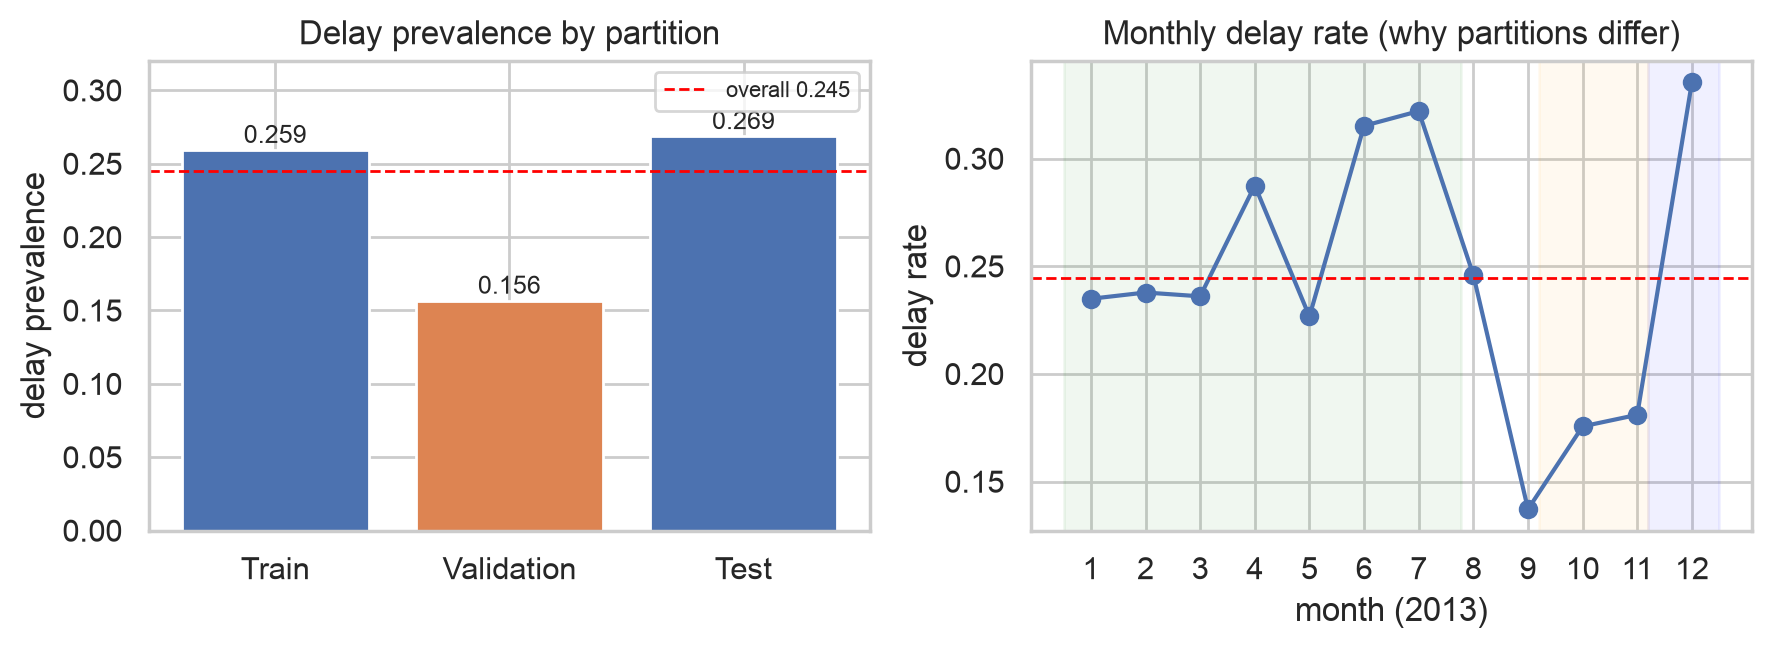
\includegraphics[width=\columnwidth]{eda-prevalence}
  \caption{Delay prevalence by partition (left) and the 2013 monthly delay-rate
  trend (right). The chronological split places the low-delay autumn months in
  validation, so partition prevalences differ by design.}
  \label{fig:prevalence}
\end{figure}

Exploratory analysis, conducted on the training partition only, surfaces the
structure the features (and embeddings) are designed to exploit
(Figs.~\ref{fig:target}--\ref{fig:distance}):
\begin{itemize}
  \item \textbf{Time of day.} Delay risk rises monotonically from roughly
  $10.5\%$ for early-morning departures to about $40\%$ late in the evening, as
  delays accumulate and cascade through the day.
  \item \textbf{Seasonality.} Summer is worst (July $\approx 32\%$), September
  best ($\approx 16\%$), reflecting weather and peak-travel load.
  \item \textbf{Day of week.} Weekdays ($27.8\%$) exceed weekends ($20.4\%$).
  \item \textbf{Carrier.} Delay propensity varies widely by operator, from
  $\approx 14\%$ to $\approx 41\%$.
  \item \textbf{Origin.} EWR ($27.9\%$) $>$ JFK ($25.5\%$) $>$ LGA ($24.0\%$),
  and delay risk also varies sharply at the finer route level
  (Fig.~\ref{fig:originroute}).
  \item \textbf{Distance.} Delay rate is largely flat across distance bands and
  dips only for the longest hauls (Fig.~\ref{fig:distance}), confirming that raw
  distance is a weak standalone signal and motivating the route and historical
  features instead.
\end{itemize}

\begin{figure}[!t]
  \centering
  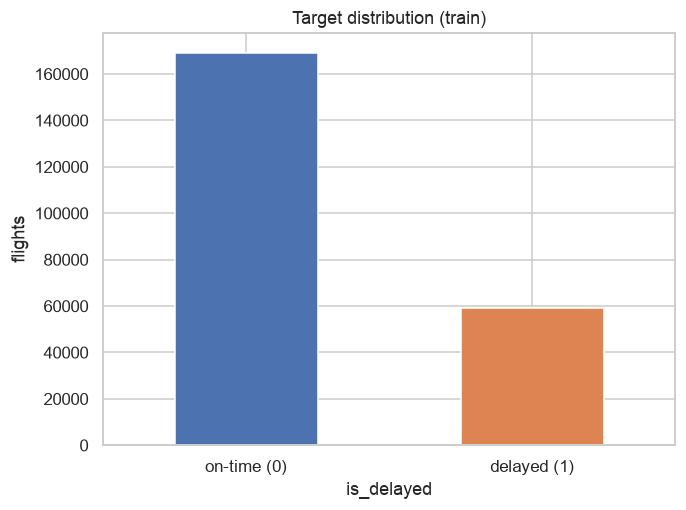
\includegraphics[width=0.78\columnwidth]{eda-target}
  \caption{Target class balance: delayed versus on-time arrivals. The minority
  (delayed) class motivates Average Precision and class weighting.}
  \label{fig:target}
\end{figure}

\begin{figure}[!t]
  \centering
  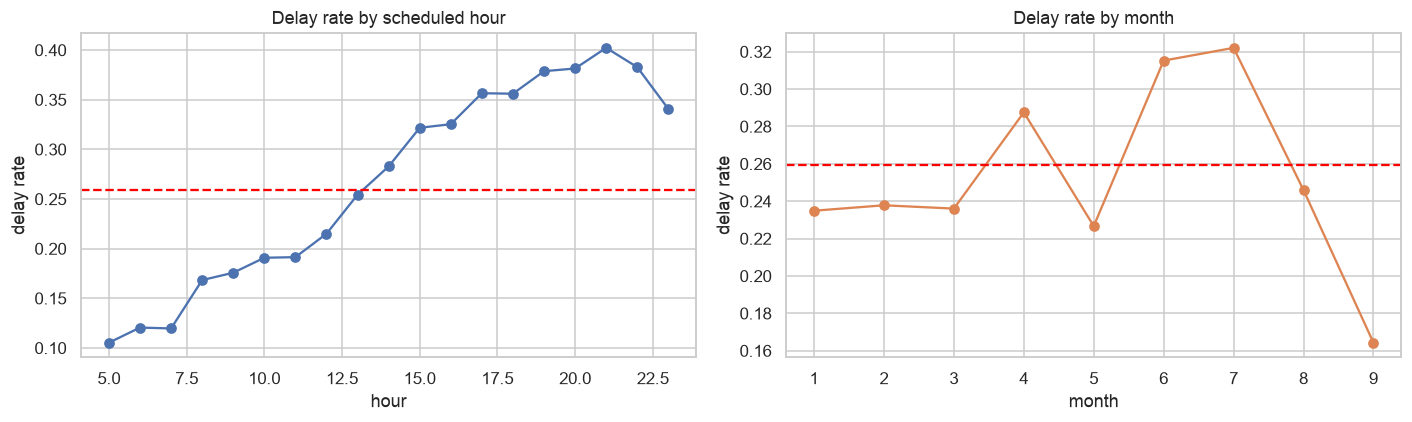
\includegraphics[width=\columnwidth]{eda-hourmonth}
  \caption{Delay rate by scheduled hour and month, exposing the strong
  time-of-day and seasonal structure exploited by the temporal features and the
  cyclic inputs reused by the Phase~2 MLP.}
  \label{fig:hourmonth}
\end{figure}

\begin{figure}[!t]
  \centering
  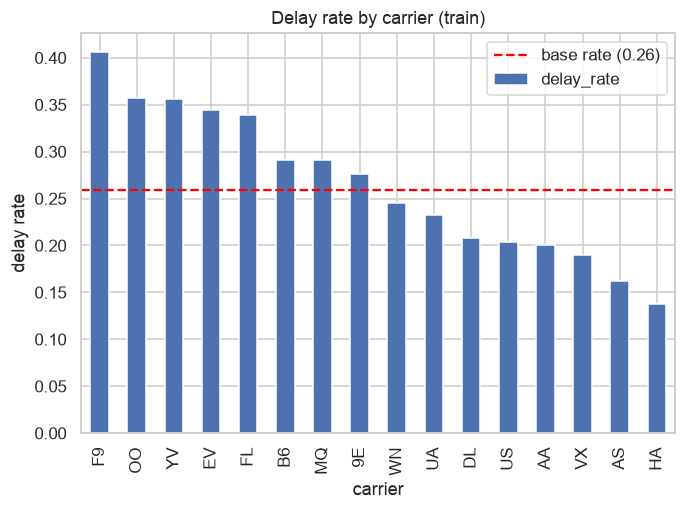
\includegraphics[width=\columnwidth]{delay-carrier}
  \caption{Delay rate by carrier. Operator-level variation motivates the carrier
  historical-delay features and the carrier entity embedding.}
  \label{fig:carrier}
\end{figure}

\begin{figure}[!t]
  \centering
  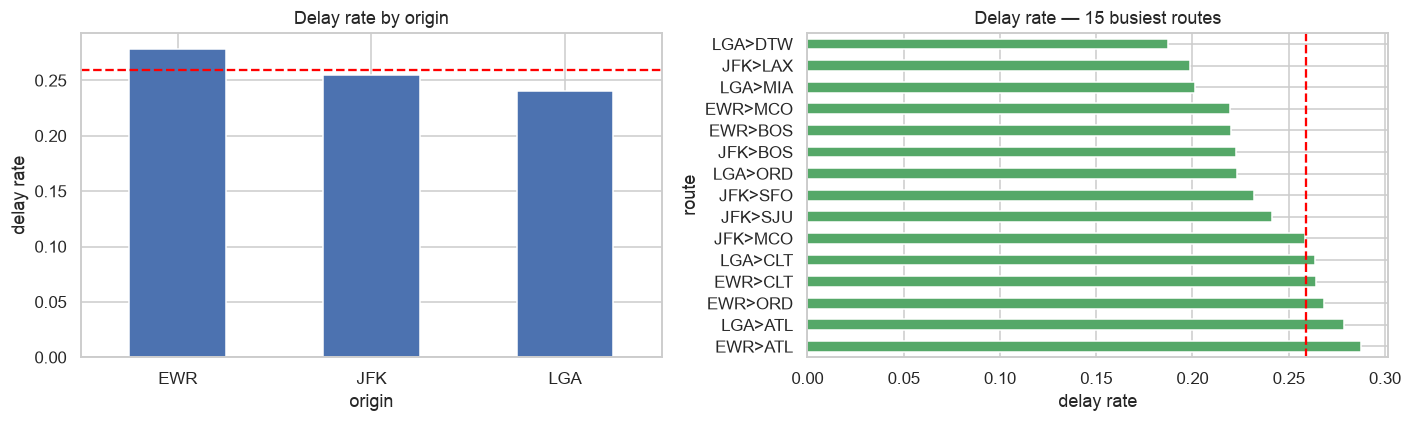
\includegraphics[width=\columnwidth]{delay-origin-route}
  \caption{Delay rate by origin airport (left) and across the fifteen busiest
  origin$\rightarrow$destination routes (right), each against the overall base
  rate (dashed). Route-level spread of roughly $19\%$ to $29\%$ motivates the
  route and route-historical features.}
  \label{fig:originroute}
\end{figure}

\begin{figure}[!t]
  \centering
  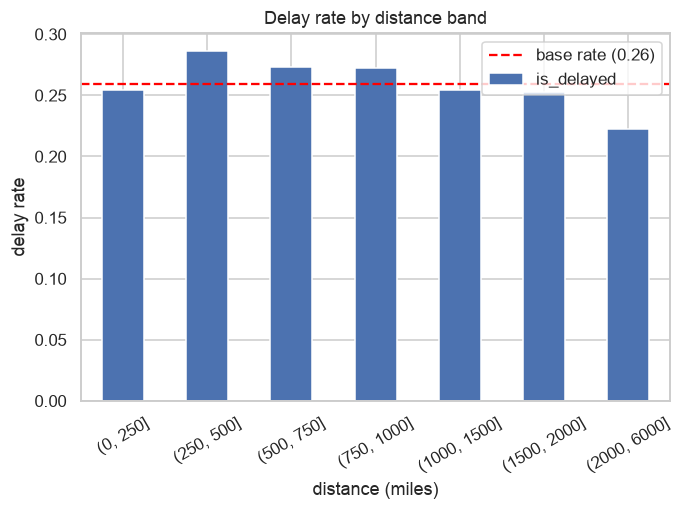
\includegraphics[width=0.82\columnwidth]{delay-distance}
  \caption{Delay rate by binned flight distance. The near-flat profile shows
  distance alone carries little signal, so it enters only as context for the
  route encoding.}
  \label{fig:distance}
\end{figure}

\section{Feature Engineering}
\label{sec:features}
The canonical frozen model uses 31 features derived from the schedule and
historical outcomes on prior calendar dates. Two additional schedule-derived
airport-load proxies form a 33-feature variant used only in a validation
ablation, not in the held-out test evaluation. The feature engines are
documented and unit-tested, and the same $31$-feature contract is consumed
unchanged by the Phase~2 neural model.

\subsection{Temporal features}
Calendar signals (\code{day\_of\_week}, \code{is\_weekend}, \code{season}) are
augmented with a \emph{cyclic} encoding of hour, month and weekday. A raw integer
hour misleads a model because it places $23{:}00$ twenty-three units from
$00{:}00$, although they are one hour apart. Mapping each periodic value $x$ with
period $P$ onto a circle,
\begin{equation}
x \mapsto \left(\sin\tfrac{2\pi x}{P},\ \cos\tfrac{2\pi x}{P}\right),
\end{equation}
restores the true adjacency (Fig.~\ref{fig:cyclic}); linear models in particular
benefit, and the MLP ingests these cyclic inputs directly.

\begin{figure}[!t]
  \centering
  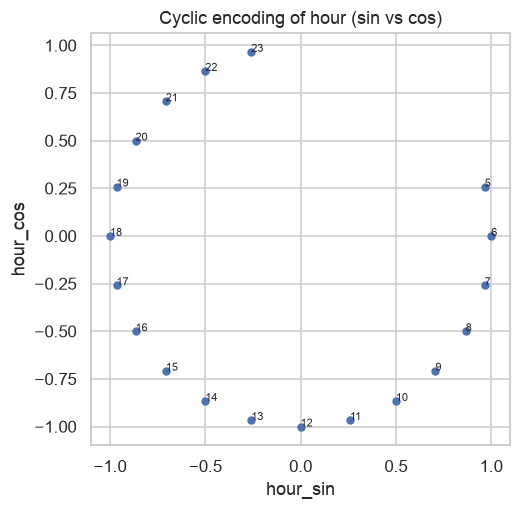
\includegraphics[width=0.82\columnwidth]{eda-cyclic}
  \caption{Cyclic hour encoding: hour $23$ sits adjacent to hour $0$ on the
  circle, unlike the raw integer representation.}
  \label{fig:cyclic}
\end{figure}

\subsection{Route features}
Static route descriptors encode the corridor and its length: the
origin$\rightarrow$destination identifier, a binned \code{distance\_band}, a
long-haul flag ($\geq 1500$ miles) and $\log(1+\text{distance})$ to compress the
heavy tail (the raw distance signal being weak, Fig.~\ref{fig:distance}). These
are fixed regardless of outcome and so introduce no leakage.

\subsection{Historical delay features}
For each carrier, origin, destination and route we compute a historical delay
rate and flight count from \emph{previous calendar dates only}, using a shifted
cumulative aggregation so that same-day and future observations are never
included. These prior-date rates correlate with the target and summarise
congestion and operational reliability that the static features cannot. Among
them, the carrier and route prior-date rates correlate most strongly with the
target (Fig.~\ref{fig:histcorr}), consistent with the operator- and
corridor-level structure seen in the exploratory analysis. We document openly
that this guarantees prior-date ordering but not the \emph{exact} availability of
each outcome at the precise prediction instant; availability-time leakage
therefore remains a stated caveat.

\begin{figure}[!t]
  \centering
  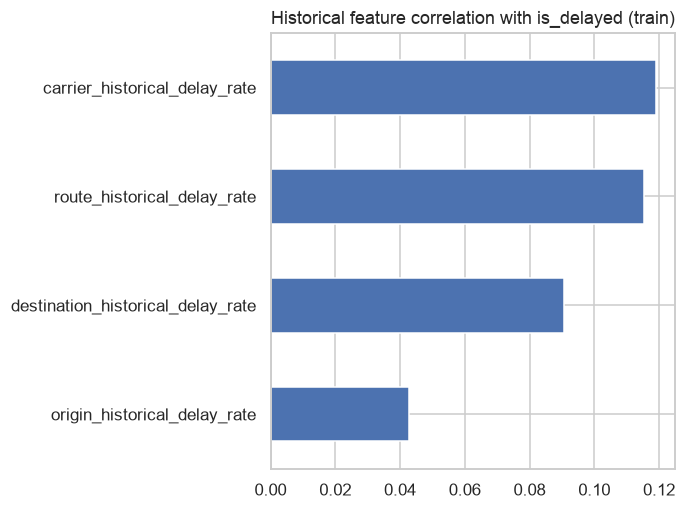
\includegraphics[width=0.9\columnwidth]{eda-histcorr}
  \caption{Pearson correlation of each prior-date historical delay rate with the
  target on the training partition. Carrier- and route-level histories are the
  most informative.}
  \label{fig:histcorr}
\end{figure}

\subsection{Airport congestion features}
To probe schedule-based airport-load proxies beyond the historical volume
features above, we examine two schedule-derived counts:
\code{origin\_hourly\_departures}, the number of flights scheduled to depart the
same origin in the same (date, hour), and \code{dest\_hourly\_arrivals}, the
analogous scheduled arrival load at the destination. The counts use the
NYC-origin timetable, not all airport operations. These are schedule-based
proxies, not measurements of realized congestion. A validation-only ablation
found small marginal differences, but does not establish that congestion is
unimportant on a larger or more complete airport dataset. The proxies are
excluded from the canonical 31-feature held-out evaluation.

\subsection{The pre-departure allowlist}
A single feature contract admits only approved predictors into the design matrix
and blocks the target, every post-departure column, and identifiers. The
canonical \code{full} allowlist uses schedule, route and historical columns; the
separate \code{full\_congestion} validation variant additionally admits the two
congestion proxies. The contract is enforced in code and tests, but prior-date
outcome availability at the exact prediction timestamp remains an unverified
assumption.

\section{Methodology}
\label{sec:method}
\subsection{Chronological split and calibration windows}
The data are partitioned by \emph{distinct calendar date} into train/validation/
test at $70/15/15$, so all flights on a date stay together and training dates
strictly precede validation dates, which precede test dates. For calibration,
the training period is split again in time: the earliest $80\%$ of training dates
fit the base estimator and preprocessing (the \emph{base-train} window), and the
remaining $20\%$ fit the calibrator (the \emph{calibration} window). No
calibration-window label ever fits a base estimator. The resulting windows are
summarised in Table~\ref{tab:windows}.

\begin{table}[!t]
  \caption{Chronological windows (2013), verified against the dataset SHA-256.}
  \label{tab:windows}
  \centering
  \begin{tabular}{lrll}
    \toprule
    Window & $n$ & First & Last \\
    \midrule
    Base train        & $181{,}405$ & 2013-01-01 & 2013-07-23 \\
    Calibration        & $46{,}894$  & 2013-07-24 & 2013-09-12 \\
    Validation         & $50{,}466$  & 2013-09-13 & 2013-11-06 \\
    Test (held out)    & $48{,}581$  & 2013-11-07 & 2013-12-31 \\
    \bottomrule
  \end{tabular}
\end{table}

\subsection{Models}
Two classifiers share the identical training rows and feature contract:
\begin{itemize}
  \item \textbf{Logistic Regression} with \code{class\_weight=} \code{"balanced"}
  to counter the class imbalance.
  \item \textbf{Tuned XGBoost} with parameters selected by training-only
  chronological cross-validation: $250$ trees, max depth $6$, learning rate
  $0.03$, minimum child weight $10$, subsample $0.90$, column subsample $0.75$,
  $L_2$ regularisation $10$, and \code{scale\_pos\_weight}$\,\approx 2.86$ for
  imbalance.
\end{itemize}
This XGBoost configuration was selected by \code{RandomizedSearchCV} over eight
sampled candidates on the \emph{training data only}, scored with three expanding
chronological folds grouped by whole flight dates and separated by a one-date
embargo so that no fold shares a date across the train/validation boundary; the
held-out test set was not used in this search.

\subsection{Calibration}
Each model's calibration-window scores are mapped by three candidates---raw
(identity), sigmoid (Platt), and isotonic---and the variant minimising validation
Brier score (log loss as tie-break) is selected. Calibrators are fit strictly on
the calibration window; validation and test labels never fit them.

\subsection{Threshold selection and the frozen protocol}
A single operating threshold per model is chosen on validation (maximising
$F_1$). The selected calibration map and threshold, the fitted estimators, the
dataset hash and the dependency versions are then \emph{frozen} to disk. Only
after this does the final stage load the frozen objects and evaluate the held-out
test set; it cannot refit or reselect. The published frozen results were
subsequently reproduced for an audit without changing any modelling decision.
Because this calendar period was also used in an earlier pre-congestion
experiment, it must not be described as a test set that was never previously
inspected.

\section{Classical Results}
\label{sec:classical-results}
\subsection{Validation}
Table~\ref{tab:val} reports validation performance at the frozen thresholds with
the selected (isotonic) calibration for both models. Ranking is similar; both
models have low precision ($\approx 22\%$) at their operating points, reflecting
the difficulty of the task. ROC and PR curves appear in
Figs.~\ref{fig:roc}--\ref{fig:pr}, and the confusion matrices at the frozen
thresholds in Fig.~\ref{fig:confusion}. On validation alone the balanced LR in
fact edges XGBoost on AP and ROC-AUC, but the two differences are tiny and, as
the date-block bootstrap below shows, not statistically distinguishable; we
therefore defer the model choice to the held-out test
(Section~\ref{sec:classical-results}\,C), where XGBoost is the stronger candidate
on every metric. Both operating points favour recall over precision---catching
roughly $60\%$ of true delays at the cost of a large false-alarm count---which is
the intended behaviour under class weighting and is exactly what the cost
analysis of Section~\ref{sec:resched} later prices.

\begin{figure}[!t]
  \centering
  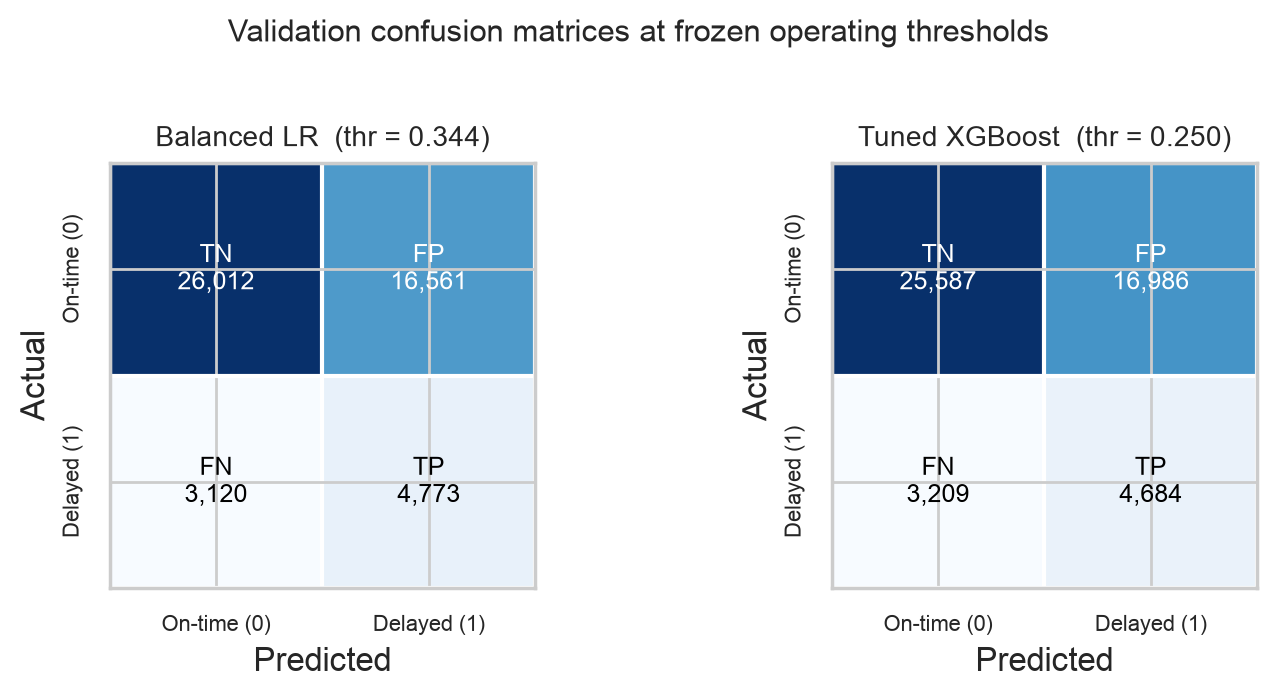
\includegraphics[width=\columnwidth]{confusion}
  \caption{Validation confusion matrices at the frozen operating thresholds for
  the two classical models. Both recover a majority of true delays (high recall)
  while incurring many false positives, consistent with their low operating
  precision.}
  \label{fig:confusion}
\end{figure}

\begin{table}[!t]
  \caption{Validation metrics (isotonic calibration; frozen thresholds).}
  \label{tab:val}
  \centering
  \setlength{\tabcolsep}{4pt}
  \resizebox{\columnwidth}{!}{%
  \begin{tabular}{lrrrrrr}
    \toprule
    Model & Thr. & AP & ROC-AUC & Prec. & Rec. & Brier \\
    \midrule
    Balanced LR    & $0.344$ & $0.223$ & $0.636$ & $0.224$ & $0.605$ & $0.151$ \\
    Tuned XGBoost  & $0.250$ & $0.213$ & $0.628$ & $0.216$ & $0.593$ & $0.137$ \\
    \bottomrule
  \end{tabular}}
\end{table}

\begin{figure}[!t]
  \centering
  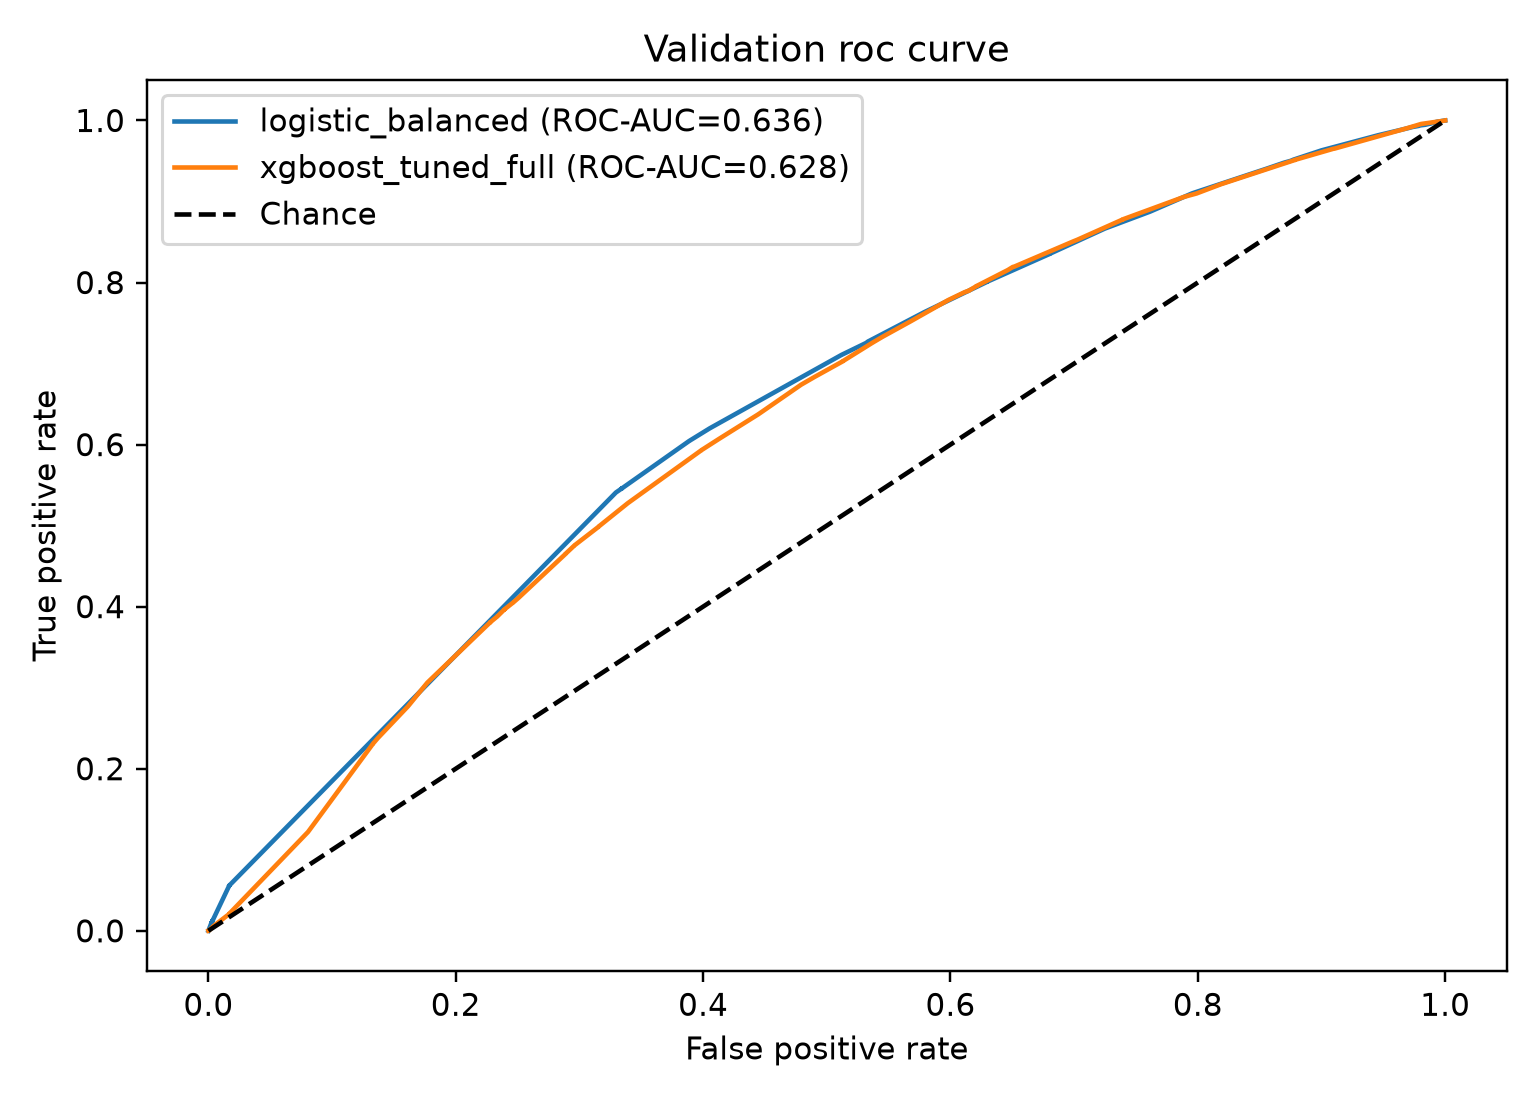
\includegraphics[width=\columnwidth]{val-roc}
  \caption{Validation ROC curves for the classical models. Discrimination is
  modest in absolute terms (ROC-AUC $\approx 0.63$--$0.64$).}
  \label{fig:roc}
\end{figure}

\begin{figure}[!t]
  \centering
  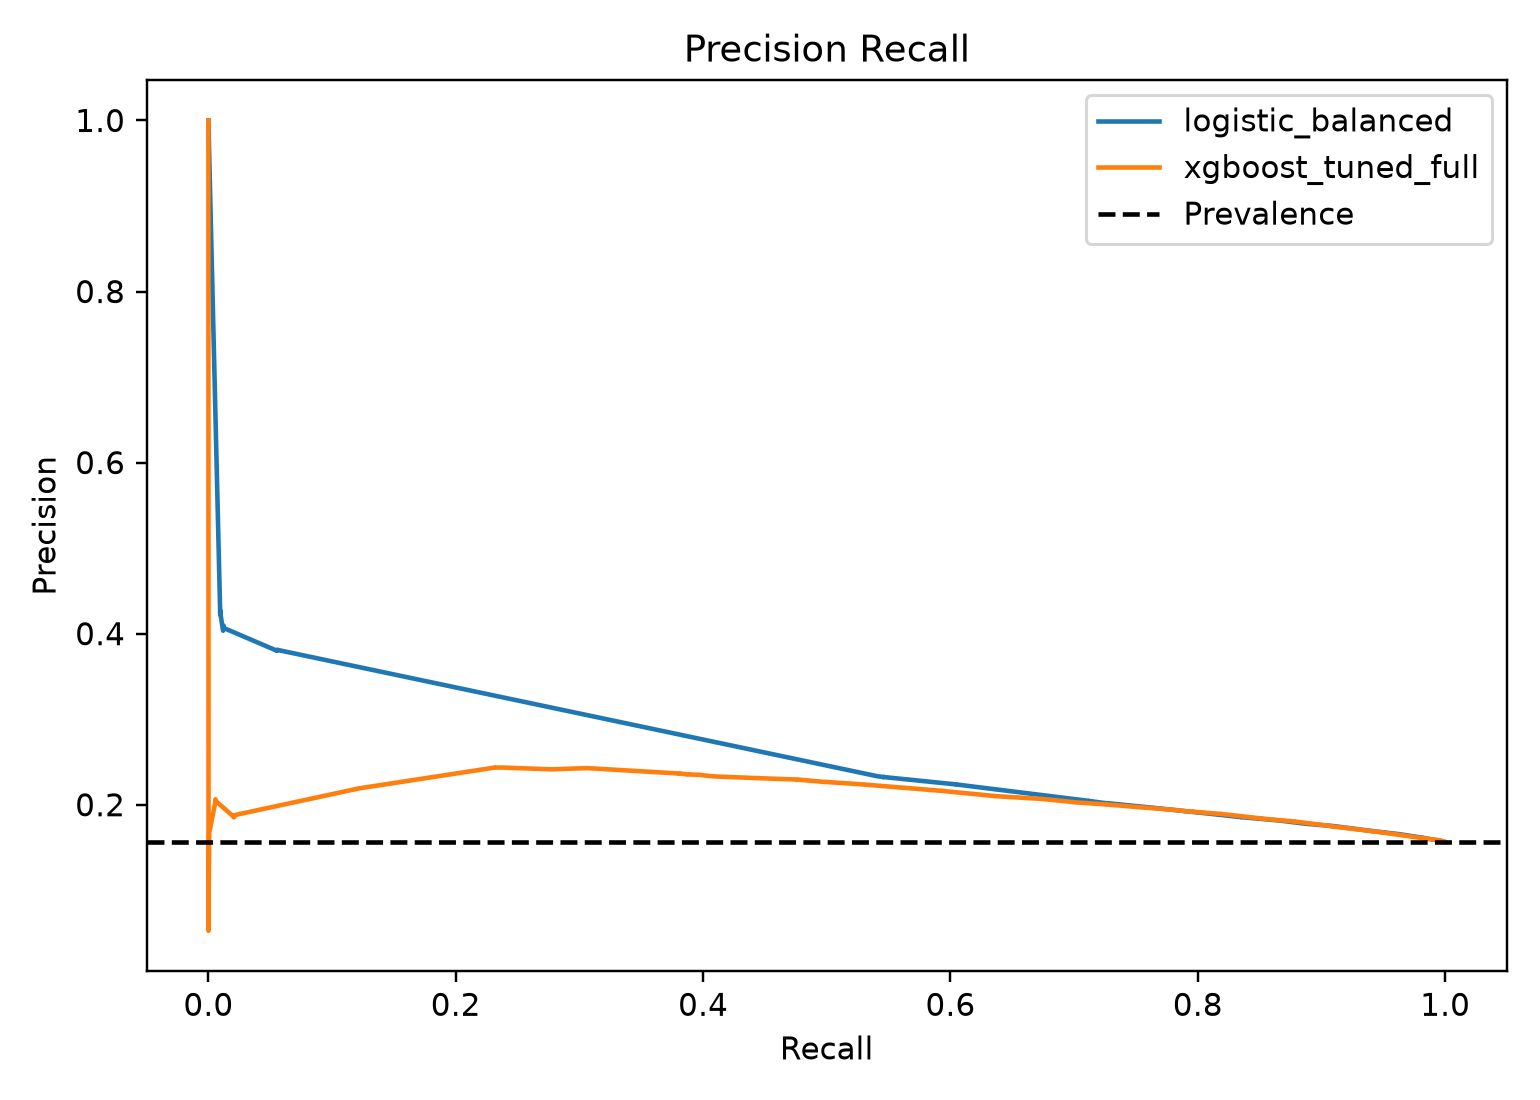
\includegraphics[width=\columnwidth]{val-pr}
  \caption{Validation precision--recall curves against the prevalence no-skill
  reference.}
  \label{fig:pr}
\end{figure}

\subsection{Calibration quality}
Isotonic regression minimises validation Brier and log loss for both models and
is selected. A proper-score audit, however, tempers any success claim: a constant
predictor set to the late-training prevalence attains a Brier of $0.138$, which
the balanced-LR isotonic probabilities ($0.151$) \emph{fail} to beat and the
XGBoost isotonic probabilities ($0.137$) beat only narrowly. Table~\ref{tab:calib}
reports the proper scores and the mean predicted probability for both models
before and after calibration: calibration slashes Brier and log loss, yet the
calibrated mean prediction ($0.23$--$0.31$) still sits above the observed
validation prevalence ($0.156$), i.e.\ both models over-predict on this
lower-prevalence window. The XGBoost reliability diagram
(Fig.~\ref{fig:reliability-xgb}) is reasonable but not strong.

\begin{table}[!t]
  \caption{Validation calibration quality (observed prevalence $0.156$;
  prevalence-baseline Brier $0.138$). Lower Brier/log loss is better; a
  well-calibrated mean prediction would match the observed prevalence.}
  \label{tab:calib}
  \centering
  \setlength{\tabcolsep}{4pt}
  \begin{tabular}{llrrr}
    \toprule
    Model & Variant & Brier & Log loss & Mean pred. \\
    \midrule
    Balanced LR   & raw       & $0.522$ & $1.396$ & $0.782$ \\
    Balanced LR   & isotonic  & $0.151$ & $0.482$ & $0.305$ \\
    Tuned XGBoost & raw       & $0.306$ & $0.860$ & $0.540$ \\
    Tuned XGBoost & isotonic  & $\mathbf{0.137}$ & $\mathbf{0.443}$ & $0.231$ \\
    \bottomrule
  \end{tabular}
\end{table}

\begin{figure}[!t]
  \centering
  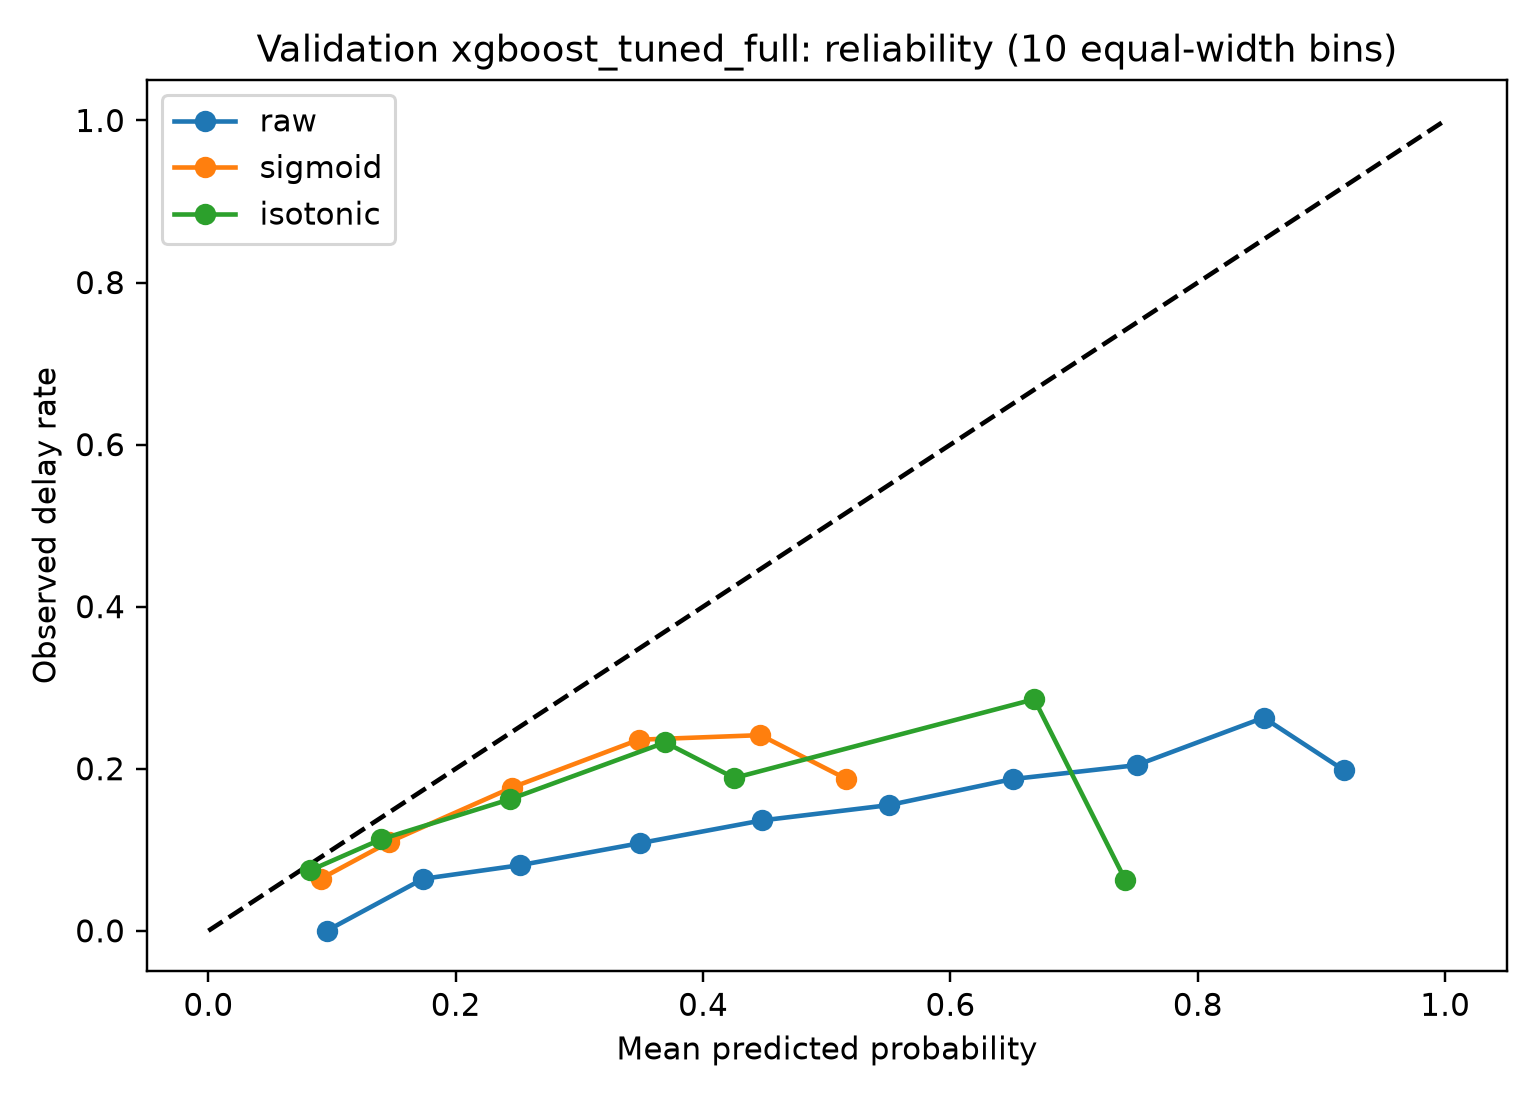
\includegraphics[width=0.9\columnwidth]{xgb-reliability}
  \caption{Validation reliability diagram for the calibrated XGBoost model (ten
  equal-width bins).}
  \label{fig:reliability-xgb}
\end{figure}

\subsection{Held-out test}
The frozen 31-feature test (Table~\ref{tab:test}) favours XGBoost on AP, ROC-AUC,
precision, recall and $F_1$. Because prevalence differs between validation
($0.156$) and test ($0.269$), the two sets' PR-based metrics are not directly
comparable as measures of improvement. A paired date-block bootstrap on
validation (300 resamples) gives differences (XGBoost minus LR) whose $95\%$
intervals include zero (e.g.\ AP $[-0.027, 0.011]$), so the ranking advantage is
descriptive rather than statistically established. These are the frozen baselines
the Phase~2 MLP and hybrid must beat.

\begin{table}[!t]
  \caption{Held-out test metrics for the frozen 31-feature models.}
  \label{tab:test}
  \centering
  \setlength{\tabcolsep}{4pt}
  \resizebox{\columnwidth}{!}{%
  \begin{tabular}{lrrrrr}
    \toprule
    Model & AP & ROC-AUC & Prec. & Rec. & $F_1$ \\
    \midrule
    Balanced LR    & $0.294$ & $0.544$ & $0.296$ & $0.488$ & $0.369$ \\
    Tuned XGBoost  & $\mathbf{0.337}$ & $\mathbf{0.599}$ & $\mathbf{0.335}$ & $\mathbf{0.532}$ & $\mathbf{0.411}$ \\
    \bottomrule
  \end{tabular}}
\end{table}

\subsection{Feature importance}
The tuned XGBoost model's gain-importance ranking (Fig.~\ref{fig:importance}) is
dominated by time-of-day signals: scheduled \code{hour}, its cyclic
\code{hour\_sin} encoding and \code{sched\_dep\_time} account for the largest
share, followed by the \code{season} flag and a high-delay carrier indicator.
This agrees with the exploratory finding that delay risk is primarily driven by
when a flight departs (Fig.~\ref{fig:hourmonth}), and confirms that the
engineered temporal features carry real model weight rather than mere decoration.
Importance here is model-relative and does not imply causation; correlated
calendar features can share or dilute one another's attributed gain.

\begin{figure}[!t]
  \centering
  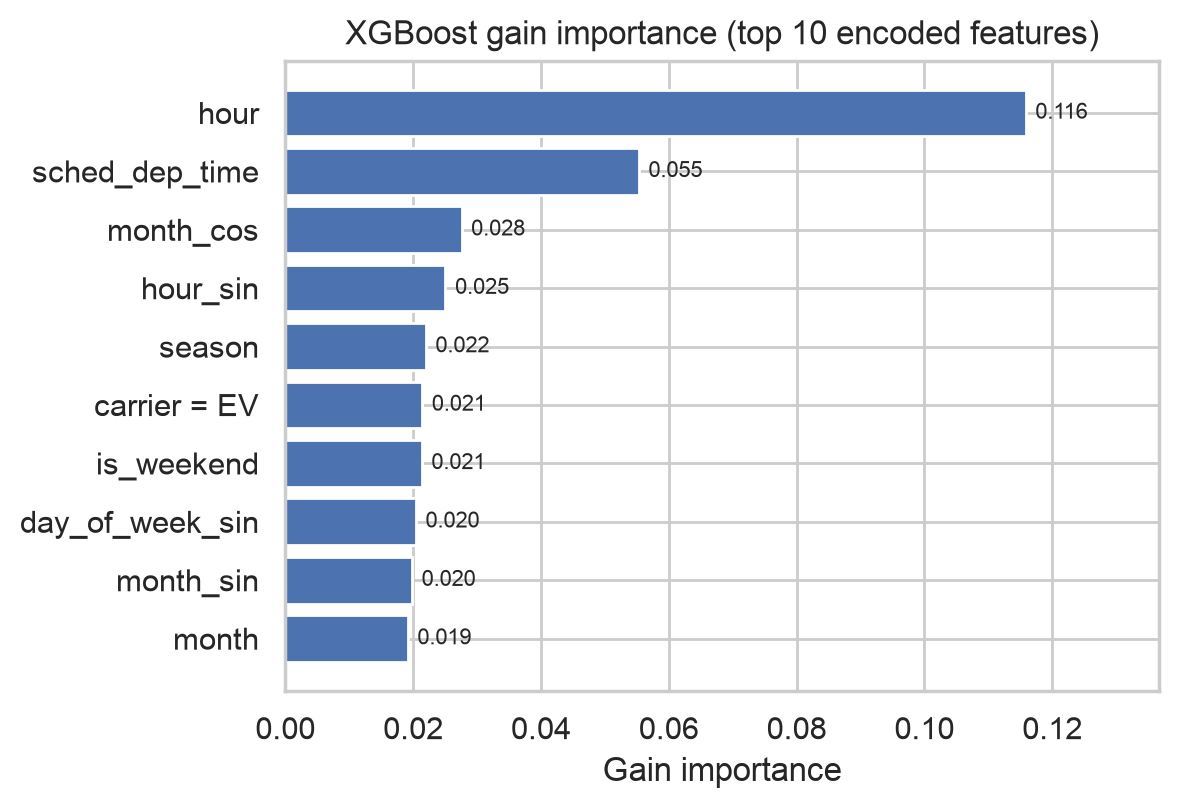
\includegraphics[width=0.95\columnwidth]{xgb-importance}
  \caption{Gain importance for the ten most influential encoded features in the
  early-training fit of the frozen XGBoost model. Time-of-day terms dominate,
  matching the exploratory structure.}
  \label{fig:importance}
\end{figure}

\section{Offline Rescheduling What-If Analysis}
\label{sec:resched}
\subsection{Cost model}
We ask, retrospectively, what the net operational cost would have been had a
proactive rescheduling action been taken on flights whose calibrated delay
probability exceeds a threshold. Per flight we assume homogeneous costs: $C_d$
for an unmitigated delay, $C_a$ for taking the action (paid whenever we act), and
a recovery fraction $r\in[0,1]$ of the delay cost avoided when we act on a flight
that truly delays. The realised cost by decision $a$ and outcome $y$ is
\begin{center}
\begin{tabular}{lcc}
\toprule
 & $y=0$ (on time) & $y=1$ (delayed) \\
\midrule
$a=0$ (no action) & $0$ & $C_d$ \\
$a=1$ (action)    & $C_a$ & $C_a + (1-r)C_d$ \\
\bottomrule
\end{tabular}
\end{center}
These assumptions---homogeneous per-flight costs, independent flights, a single
binary action, and no network feedback---are strong and are declared as
limitations; no operational cost has been approved, so all quantities are
expressed relative to $C_d$.

\subsection{Closed-form net benefit and the optimal threshold}
For a policy that acts on $\mathrm{tp}$ true delays and $\mathrm{fp}$ on-time
flights, the saving relative to the no-action status quo is
\begin{equation}
\text{net} = \mathrm{tp}\,(r\,C_d - C_a) - \mathrm{fp}\,C_a,
\label{eq:net}
\end{equation}
a cost-sensitive generalisation of decision-curve net benefit. Acting on a flight
has non-negative expected value exactly when its calibrated probability $p$
satisfies $p\,r\,C_d \geq C_a$, giving the \emph{cost-optimal action threshold}
\begin{equation}
\tau^\star = \frac{C_a}{r\,C_d} = \frac{C_a/C_d}{r}.
\label{eq:tau}
\end{equation}
The decision boundary is thus read directly from the cost assumptions---which is
precisely why calibration matters operationally, as only a well-calibrated $p$
makes $\tau^\star$ the right place to cut.

\subsection{Sensitivity and findings}
Because real costs are unknown, we sweep the cost ratio $C_a/C_d$ at $r=0.8$ on
the validation partition (preserving the held-out test), evaluating each model at
its optimal $\tau^\star$ (Table~\ref{tab:sweep}, Fig.~\ref{fig:netbenefit}).

\begin{table}[!t]
  \caption{Rescheduling sensitivity: net saving per flight (units of $C_d$) at
  the cost-optimal threshold, $r=0.8$. ``$+$'' beats no action.}
  \label{tab:sweep}
  \centering
  \begin{tabular}{rrrr}
    \toprule
    $C_a/C_d$ & $\tau^\star$ & Balanced LR & Tuned XGBoost \\
    \midrule
    $0.05$ & $0.063$ & $+0.075$ & $+0.075$ \\
    $0.10$ & $0.125$ & $+0.025$ & $+0.034$ \\
    $0.15$ & $0.188$ & $-0.016$ & $+0.005$ \\
    $0.20$ & $0.250$ & $-0.049$ & $-0.012$ \\
    $0.25$ & $0.313$ & $-0.056$ & $-0.018$ \\
    \bottomrule
  \end{tabular}
\end{table}

\begin{figure}[!t]
  \centering
  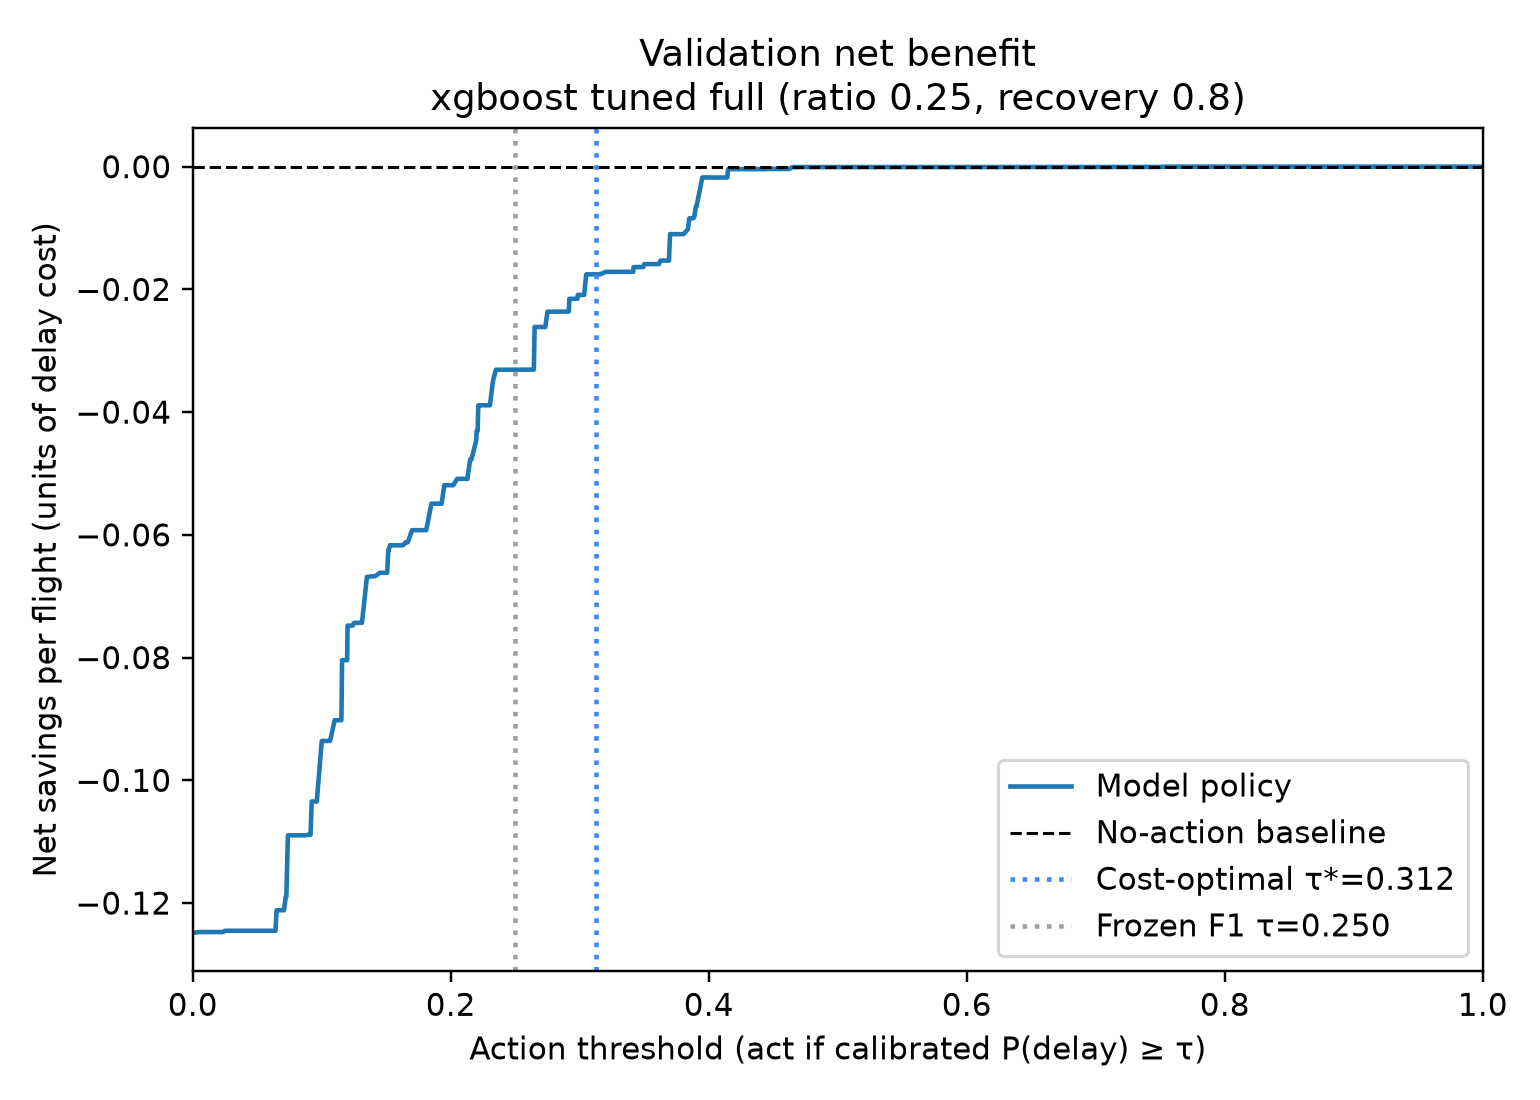
\includegraphics[width=\columnwidth]{xgb-netbenefit}
  \caption{Validation XGBoost net saving per flight versus action threshold
  (cost ratio 0.25 and recovery 0.8). The curve crosses the no-action line, and
  the cost-optimal $\tau^\star$ moves with the assumed cost ratio.}
  \label{fig:netbenefit}
\end{figure}

Three findings follow. First, a model-driven rule beats inaction only when the
action is cheap relative to a delay---up to $C_a/C_d\approx 0.10$ for Logistic
Regression and $\approx 0.15$ for XGBoost; beyond that, low precision makes the
false-alarm term in~\eqref{eq:net} dominate and intervention is not justified.
Second, \textbf{XGBoost has the more favourable sensitivity profile across the
meaningful cost range}---a wider contiguous positive-saving region and higher
oracle efficiency at matched cost ratios---a decision-relevant advantage the
ranking metrics alone did not make vivid. Third, even the best attainable
efficiency is modest (about $64\%$ of the perfect-foresight oracle at the
cheapest ratio), bounding what any policy built on the current probabilities can
deliver. The calibrated classical XGBoost therefore remains the basis for the
offline decision analysis.

\section{Phase 2 Dataset Contract and Leakage Audit}
\label{sec:dataset}
Phase~2 adapts the Phase~1 pipeline without changing the label definition, the
split rule, or the feature allowlist. The adapter (\code{deep\_learning.dataset})
returns NumPy arrays plus aligned comparison metadata (\code{flight\_id},
\code{flight\_date}, \code{y\_true}, \code{partition}); it performs no training,
calibration, threshold selection, or test scoring. The adapter exposes $26$
numeric features and five categorical columns; \code{carrier}, \code{origin} and
\code{dest} are embedded, while \code{route} and \code{distance\_band} are
appended as one-hot blocks.

\textbf{Leakage discipline.}
A positive allowlist blocks \code{dep\_time}, \code{dep\_delay},
\code{arr\_time}, \code{arr\_delay}, \code{air\_time}, raw labels and
identifiers. Historical features aggregate labels by entity and date and subtract
the \emph{entire current date} from cumulative totals, so neither a flight's own
label, other same-day labels, nor future-date outcomes enter its predictors.
Unit tests perturb current/future outcomes and verify that earlier inputs are
unchanged across partition boundaries. We disclose one honest caveat: date-order
safety guarantees prior-date \emph{ordering} but not the exact real-time
\emph{availability} of every previous-day outcome at the prediction instant
(overnight arrivals and publication latency can violate it). We therefore do not
claim proven deployment-time leakage freedom.

\textbf{Prevalence across the calibration boundary.}
Beyond the partition shift of Section~\ref{sec:data}, the train-calibration
window is $23.31\%$ delayed versus validation's $15.64\%$. This gap is why the
MLP's calibrator, fitted on the higher-prevalence window, later over-predicts on
validation, and why we read the validation no-skill AP as $0.156$ rather than
treating cross-window PR differences as improvements.

\section{Architecture Logic}
\label{sec:arch}
The model, \code{FlightDelayMLP}, predicts a single delay logit per flight and is
designed so that the categorical identity of a flight is \emph{learned}, not
hand-encoded.

\textbf{Batch interface.}
Each batch is a pair $(\code{x\_dense}, \code{x\_cat})$: \code{x\_dense} is a
float32 matrix of the $26$ standardised numeric features plus the one-hot
\code{route}/\code{distance\_band} blocks, in the encoder's fixed column order;
\code{x\_cat} is a long tensor of three IDs (\code{carrier}, \code{origin},
\code{dest}). The forward pass looks up the three embedding vectors, concatenates
them with \code{x\_dense}, applies each hidden linear layer followed by ReLU and
dropout, and ends in a linear layer with one output. Training uses
\code{BCEWithLogitsLoss}; probabilities are obtained by a sigmoid at inference.

\textbf{Embedding widths.}
Table widths follow a conservative square-root heuristic,
$d=\min(16,\max(2,\lceil\sqrt{c}\rceil))$ where $c$ is the known-category
cardinality. This yields compact widths---about $2$ for the three NYC origins,
$\approx 4$ for carriers, and $\approx 11$ for destinations---so the embeddings
add representational capacity without exploding parameters on a dataset this
size.

\textbf{Reserved indices (robustness).}
Index $0$ denotes a \emph{missing} category and index $1$ an \emph{unseen}
category; known training categories start at $2$. Vocabularies are fitted on
early-training data only. The unseen index~$1$ is a \code{padding\_idx} whose
vector is initialised to zero and \emph{frozen} (no gradient), so a carrier or
airport absent from the training period cannot activate untrained weights; the
missing index~$0$ stays trainable so the model can learn a representation of
missingness. This lets the model score out-of-vocabulary flights without errors,
and never discards rows.

\section{Training, Regularisation, and Reproducibility}
\label{sec:training}
The network is trained with the AdamW optimiser. Early stopping monitors
validation Average Precision with patience~$4$ and a minimum improvement of
$10^{-4}$, and the best checkpoint is restored; the test partition is never used
for early stopping or selection. Regularisation combines three mechanisms:
\emph{dropout} in the hidden layers, AdamW \emph{weight decay}, and
\emph{early stopping} on validation AP, with the frozen-zero unseen embedding
acting as a fourth, structural guard against spurious capacity.

\textbf{Why the best epoch is~1.}
The selected checkpoint stops at epoch~1. This is not a bug but a direct
consequence of the weak pre-departure signal: the model extracts essentially all
of the learnable structure in its first pass over $181{,}405$ training rows, and
further epochs only begin to overfit, so validation AP peaks immediately and
early stopping restores epoch~1. It is corroborating evidence that the ceiling
here is set by the information in pre-departure features, not by optimisation.

\textbf{Reproducibility.}
Python, NumPy and PyTorch seeds are fixed and deterministic algorithms are
requested. Repeated CPU runs in the verification environment reproduced the
exported probabilities bit-for-bit, and the committed checkpoint replays to the
saved validation probabilities within numerical tolerance
(Section~\ref{sec:validation}).

\section{Hyperparameter Search and Matched-Seed Ablation}
\label{sec:ablation}
\textbf{Selection search.}
A six-trial search (Table~\ref{tab:search}) varied one factor at a time over
learning rate, batch size, hidden widths, dropout and weight decay, each with its
own seed, and selected on validation AP alone. The published checkpoint
(dropout~$0.3$, learning rate~$0.001$, batch~$1024$, hidden widths $[128,64]$,
weight decay~$10^{-4}$, seed~$46$) scored validation AP~$0.20658$.

\begin{table}[!t]
  \caption{Selection search (one factor changed per trial; own seed).}
  \label{tab:search}
  \centering
  \setlength{\tabcolsep}{4pt}
  \resizebox{\columnwidth}{!}{%
  \begin{tabular}{clllll r}
    \toprule
    \# & LR & Batch & Hidden & Drop. & WD & Val AP \\
    \midrule
    0 & $0.001$  & $1024$ & $[128,64]$ & $0.1$ & $10^{-4}$ & $0.19939$ \\
    1 & $0.0005$ & $1024$ & $[128,64]$ & $0.1$ & $10^{-4}$ & $0.20600$ \\
    2 & $0.001$  & $512$  & $[128,64]$ & $0.1$ & $10^{-4}$ & $0.19733$ \\
    3 & $0.001$  & $1024$ & $[64,32]$  & $0.1$ & $10^{-4}$ & $0.20369$ \\
    4 & $0.001$  & $1024$ & $[128,64]$ & $0.3$ & $10^{-4}$ & $\mathbf{0.20658}$ \\
    5 & $0.001$  & $1024$ & $[128,64]$ & $0.1$ & $10^{-3}$ & $0.20578$ \\
    \bottomrule
  \end{tabular}}
\end{table}

\textbf{Why a matched-seed ablation.}
A single-seed search confounds the effect of a hyperparameter with the effect of
its random initialisation and batch order. We therefore reran all six
configurations at each of three shared seeds ($42$, $46$, $50$), subtracted the
baseline AP at the \emph{same} seed, and summarised the three paired differences
(Table~\ref{tab:ablation}). This isolates each factor's effect from seed noise
and uses the same chronological windows and early-stopping rule throughout.

\begin{table}[!t]
  \caption{Matched-seed ablation: mean validation-AP change vs.\ the same-seed
  baseline (seeds $42,46,50$).}
  \label{tab:ablation}
  \centering
  \setlength{\tabcolsep}{4pt}
  \begin{tabular}{lrrr}
    \toprule
    Change from baseline & Mean $\Delta$AP & Min & Max \\
    \midrule
    LR $0.001\!\rightarrow\!0.0005$      & $+0.004759$ & $+0.004466$ & $+0.005189$ \\
    Batch $1024\!\rightarrow\!512$       & $-0.004602$ & $-0.006085$ & $-0.003278$ \\
    Hidden $[128,64]\!\rightarrow\![64,32]$ & $+0.001489$ & $+0.000046$ & $+0.002479$ \\
    Dropout $0.1\!\rightarrow\!0.3$      & $+0.002135$ & $+0.001270$ & $+0.002942$ \\
    WD $10^{-4}\!\rightarrow\!10^{-3}$   & $+0.000027$ & $-0.000022$ & $+0.000092$ \\
    \bottomrule
  \end{tabular}
\end{table}

\textbf{Reading the ablation.}
The lower learning rate gives the largest and most consistent gain ($+0.0048$ on
average, positive at all three seeds), indicating the default rate slightly
overshoots on this smooth objective. Raising dropout to $0.3$ helps at every seed
($+0.0021$), which is why it is in the final model. A smaller batch \emph{hurts}
($-0.0046$), consistent with noisier gradient estimates on an already weak
signal. Narrower hidden widths and extra weight decay are near-neutral---and the
weight-decay effect changes sign across seeds, so it is within noise. All effects
are small in absolute terms ($\lesssim 0.005$~AP), which is itself informative:
no single knob unlocks substantially more signal, reinforcing that the ceiling is
data-limited.

\section{Hybrid Innovation: Stacked XGBoost $+$ MLP}
\label{sec:hybrid}
\textbf{Design.}
A logistic-regression meta-learner is fitted on two features---the frozen Phase~1
XGBoost probability and the Phase~2 MLP probability---using \emph{only} the
late-training \code{train\_calibration} partition, and evaluated on validation.
Both base models were trained on the early-training partition alone, so their
probabilities on the calibration rows are genuinely out-of-sample; the test
partition is never loaded. This discipline is enforced in code and asserted in
tests.

\textbf{Result.}
The hybrid's validation AP is $0.2093$ (vs.\ $0.2129$ for calibrated XGBoost and
$0.2233$ for calibrated Logistic Regression) and its Brier is $0.137145$ (vs.\
$0.137199$ for calibrated XGBoost)---a gain of just $0.000054$. A paired
calendar-day bootstrap gives an MLP-minus-XGBoost AP difference of $-0.0047$ with
a $95\%$ interval $[-0.0197, 0.0051]$ that includes zero: the two are
statistically indistinguishable in ranking.

\textbf{Why it does not help (the key diagnosis).}
Stacking can only recover signal when base models make \emph{different} errors.
Here they do not. On validation the XGBoost and MLP \emph{residuals} (observed
minus raw predicted risk) have Pearson correlation~$0.968$, their probabilities
correlate $0.907$ (Pearson) and $0.905$ (Spearman). With errors this collinear
there is almost no diversity to exploit, so the meta-learner leans almost
entirely on the stronger base model: its coefficients are $+3.49$ on XGBoost,
$-0.87$ on the MLP, intercept $-2.87$. The negligible Brier change is the
quantitative signature of a redundant second model. This is precisely the
regime~\cite{grinsztajn,shwartzziv} describe---on a feature-engineered tabular
target the deep model and the tree learn the same thing---so we report the hybrid
as a sound negative/ablation result and name representation-level
fusion~\cite{entityembed,fbgbdt} as the justified, though likely low-upside, next
step.

\section{Fair Comparison and Results}
\label{sec:eval}
\textbf{Protocol.}
Every candidate exports probabilities on the \emph{same} $50{,}466$ validation
flights with identical IDs, dates and binary labels (independently audited to
match to displayed precision, $15.6402\%$ delayed). MLP sigmoid/isotonic
calibrators are fitted only on the $46{,}894$ calibration flights; the MLP
calibration map is selected by validation Brier with a log-loss tie-break, which
chooses isotonic. Calibration and threshold choices are made on validation and
are therefore \emph{not} independent final-test claims.

\begin{table}[!t]
  \caption{Validation metrics on the $50{,}466$ aligned flights (selected
  calibration). AP/ROC-AUC higher is better; Brier/log loss/ECE lower is better.}
  \label{tab:results}
  \centering
  \setlength{\tabcolsep}{3.5pt}
  \resizebox{\columnwidth}{!}{%
  \begin{tabular}{lrrrrr}
    \toprule
    Model & AP & ROC-AUC & Brier & Log loss & ECE \\
    \midrule
    Logistic, raw        & $\mathbf{0.2532}$ & $\mathbf{0.6467}$ & $0.5219$ & $1.3959$ & $0.6255$ \\
    Logistic, isotonic   & $0.2233$ & $0.6360$ & $0.1509$ & $0.4822$ & $0.1487$ \\
    XGBoost, raw         & $0.2112$ & $0.6278$ & $0.3059$ & $0.8600$ & $0.3838$ \\
    XGBoost, isotonic    & $0.2129$ & $0.6279$ & $0.1372$ & $0.4428$ & $0.0746$ \\
    MLP, raw             & $0.2066$ & $0.6206$ & $0.2085$ & $0.5976$ & $0.2465$ \\
    MLP, isotonic        & $0.2082$ & $0.6207$ & $0.1375$ & $0.4451$ & $0.0861$ \\
    Hybrid (XGB$+$MLP)   & $0.2093$ & $0.6255$ & $\mathbf{0.1371}$ & $\mathbf{0.4411}$ & $0.0718$ \\
    \bottomrule
  \end{tabular}}
\end{table}

\textbf{Ranking.}
Table~\ref{tab:results} and Figs.~\ref{fig:dlroc}--\ref{fig:dlap} show the
headline picture: all models are close, and the deep models do \emph{not} lead.
Raw balanced Logistic Regression has the best AP/ROC-AUC but is severely
miscalibrated (see below); among calibrated models, Logistic leads on AP, then
XGBoost, then the hybrid, then the MLP. Absolute discrimination is modest
(ROC-AUC $\approx 0.62$--$0.65$), bounded by the pre-departure constraint: with no
same-day operational state, weather, or upstream-aircraft information available at
the decision point, the schedule/route/history features simply do not separate
delayed from on-time flights sharply. The AP bar chart (Fig.~\ref{fig:dlap})
makes the near-tie among calibrated models explicit against the $0.156$ no-skill
floor.

\begin{figure}[!t]
  \centering
  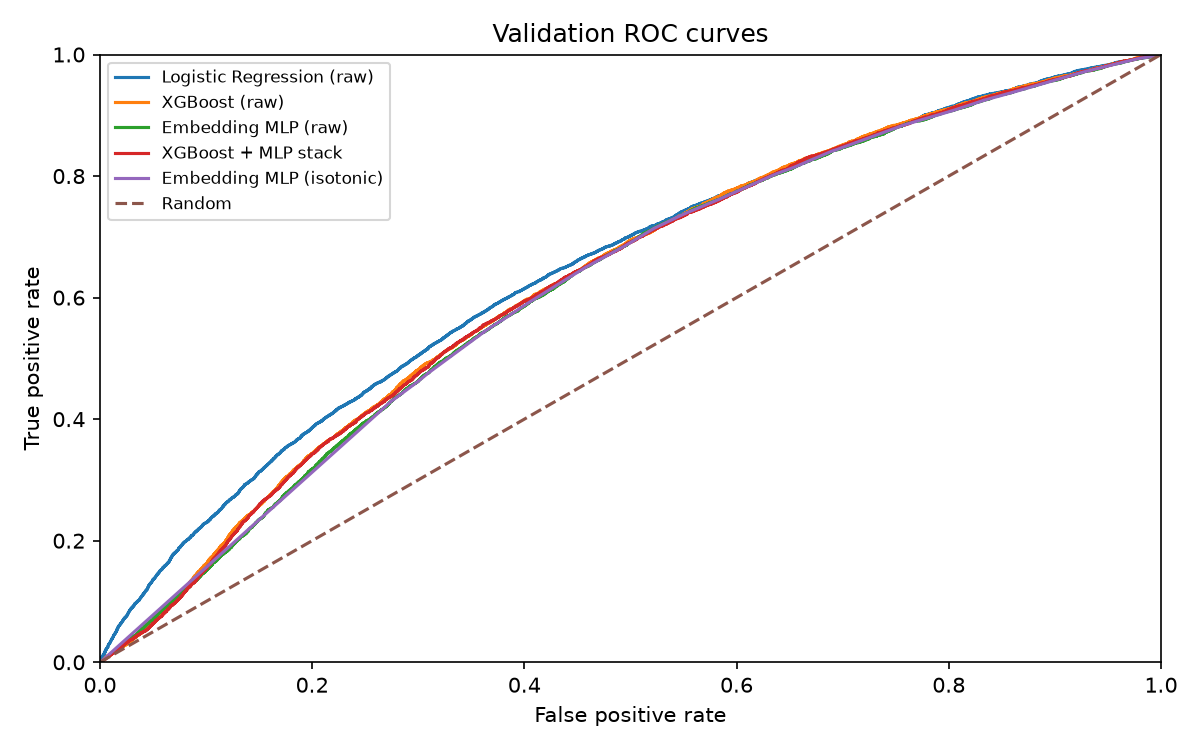
\includegraphics[width=\columnwidth]{dl-roc}
  \caption{Validation ROC curves for the Phase~2 comparison. Discrimination is
  modest in absolute terms (ROC-AUC $\approx 0.62$--$0.65$), reflecting the weak
  pre-departure signal rather than a modelling defect.}
  \label{fig:dlroc}
\end{figure}

\begin{figure}[!t]
  \centering
  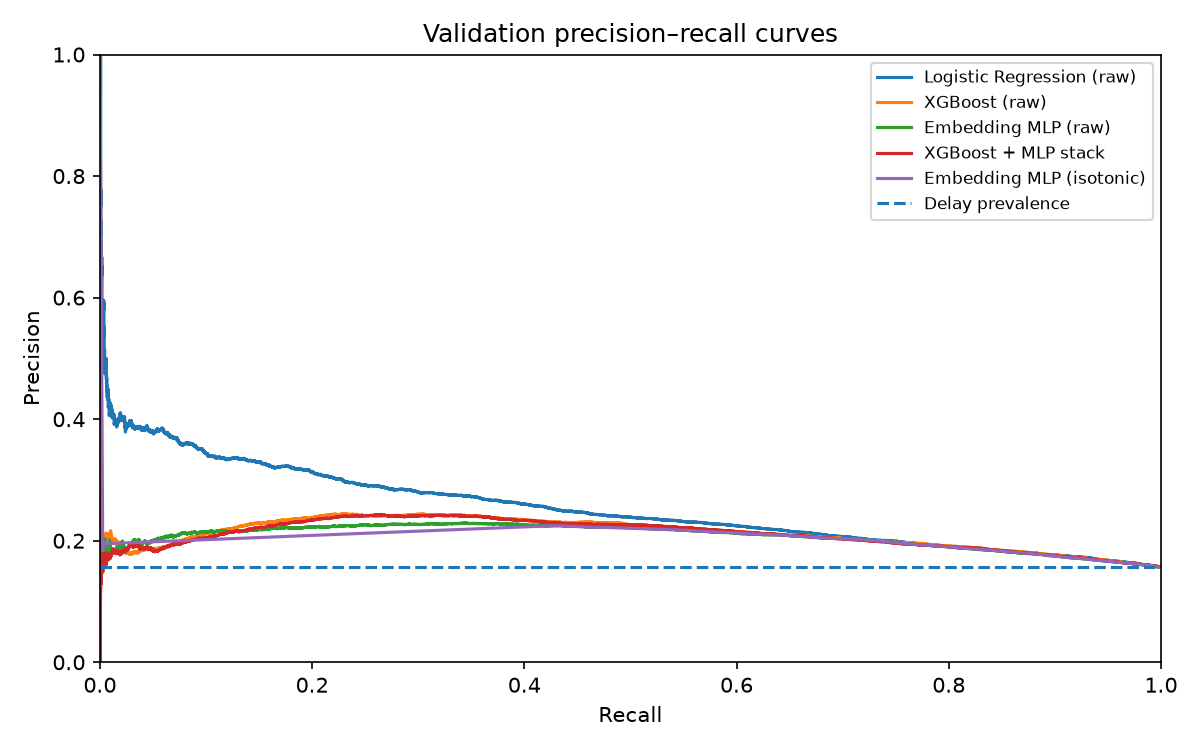
\includegraphics[width=\columnwidth]{dl-pr}
  \caption{Validation precision--recall curves against the prevalence no-skill
  reference ($0.156$). The calibrated models are nearly coincident.}
  \label{fig:dlpr}
\end{figure}

\begin{figure}[!t]
  \centering
  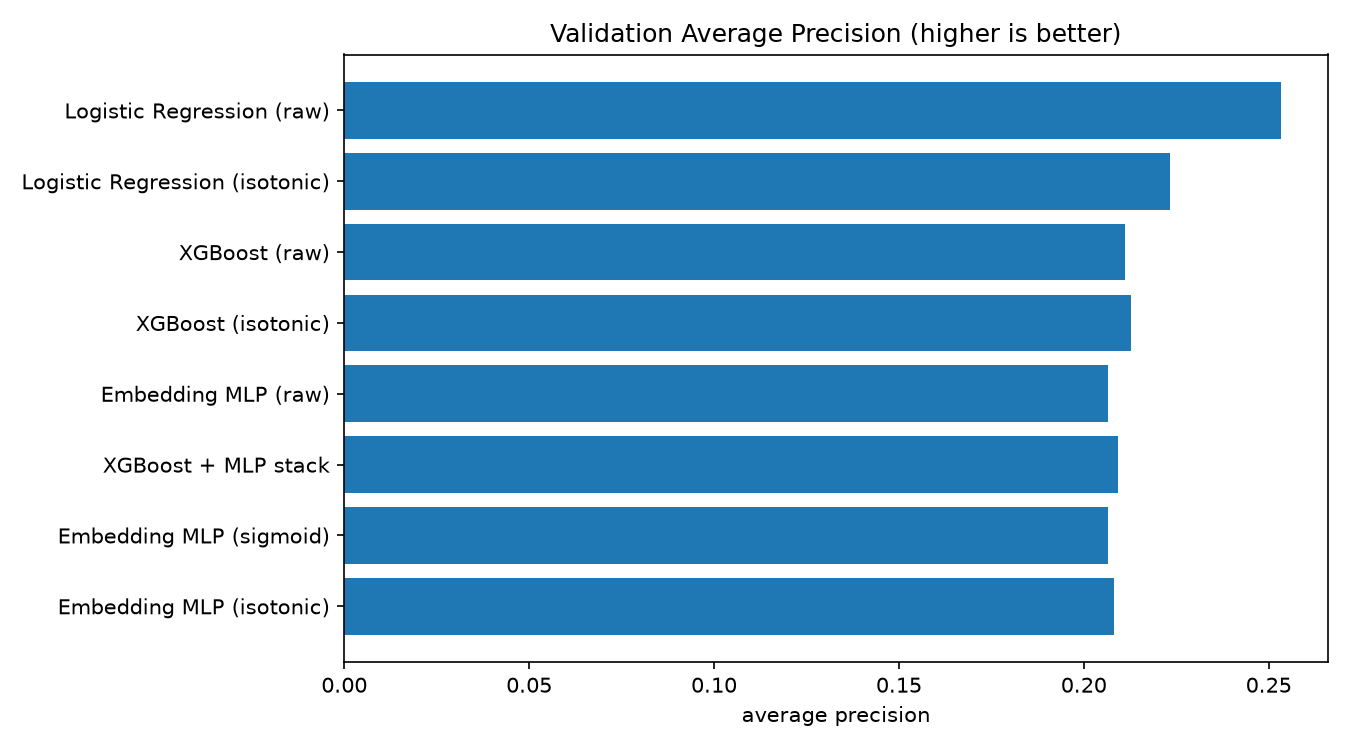
\includegraphics[width=\columnwidth]{dl-ap}
  \caption{Average Precision by model. The embedding MLP and the hybrid sit just
  below calibrated XGBoost and Logistic Regression; all cluster well above the
  no-skill floor but within a narrow band.}
  \label{fig:dlap}
\end{figure}

\subsection{Calibration quality}
\label{sec:calibration}
Isotonic calibration brings every model to Brier $\approx 0.137$
(Fig.~\ref{fig:dlbrier}), and the reliability diagram
(Fig.~\ref{fig:dlreliability}) shows the calibrated curves tracking the diagonal
far better than the raw ones. Two reasoned observations follow.

First, the \emph{raw} MLP (Brier $0.2085$) is already much better calibrated than
raw XGBoost (Brier $0.3059$, mean prediction $0.54$). The reason is training
setup: the MLP's BCE loss with no class reweighting keeps its probabilities near
the base rate, whereas XGBoost's \code{scale\_pos\_weight}$\,\approx 2.86$
deliberately inflates positive scores for ranking, which wrecks raw calibration
until isotonic repair.

Second, a proper-score audit tempers any success claim. A constant predictor set
to the train-calibration prevalence achieves Brier~$0.1378$; the calibrated MLP
($0.1375$), calibrated XGBoost ($0.1372$) and hybrid ($0.1371$) beat this
prevalence baseline only narrowly, and calibrated Logistic ($0.1509$) fails to
beat it at all. Moreover every calibrated model's mean prediction ($0.23$--$0.31$)
still exceeds the observed validation prevalence ($0.156$) because the model was
calibrated on a higher-prevalence ($0.233$) window---an honest limitation of
calibrating across a prevalence shift. The calibrated probabilities are therefore
usable but only modestly informative.

\begin{figure}[!t]
  \centering
  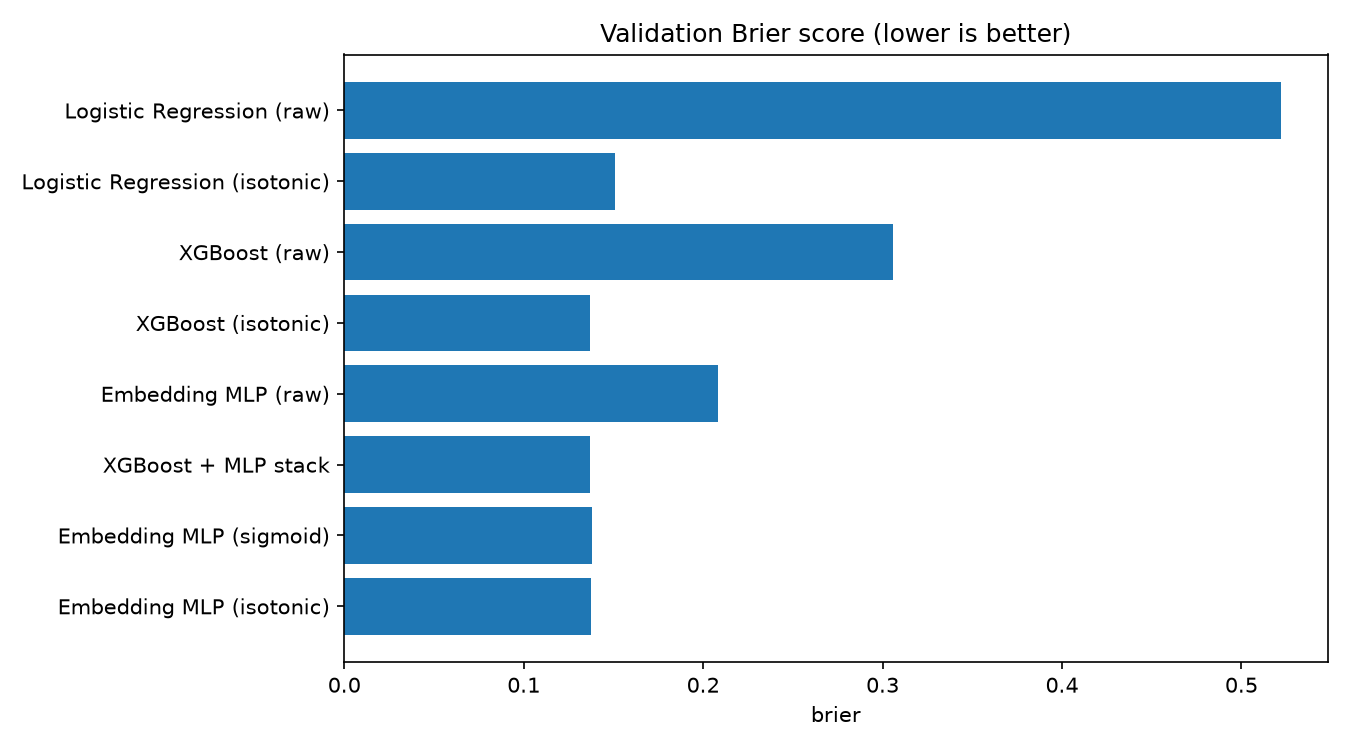
\includegraphics[width=\columnwidth]{dl-brier}
  \caption{Brier score by model. Isotonic calibration collapses the raw
  differences; all calibrated models land near $0.137$, just below the
  prevalence-baseline Brier of $0.138$.}
  \label{fig:dlbrier}
\end{figure}

\begin{figure}[!t]
  \centering
  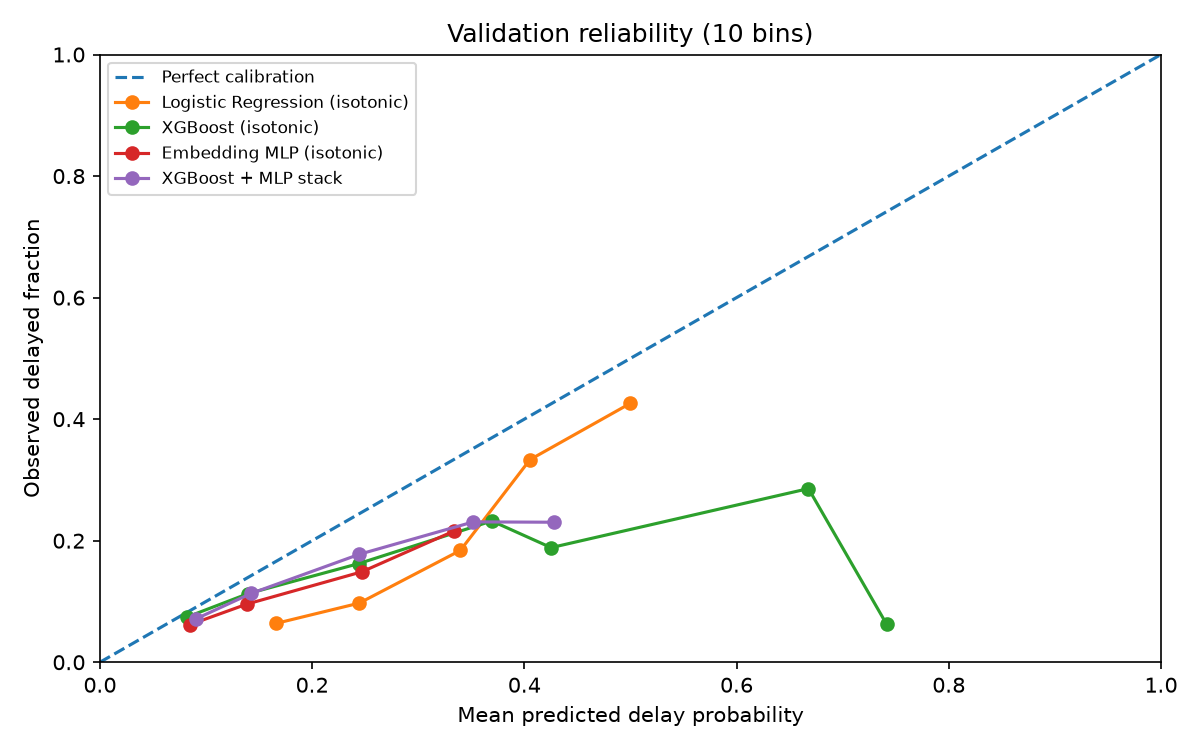
\includegraphics[width=\columnwidth]{dl-reliability}
  \caption{Validation reliability diagram for the calibrated classical models,
  the calibrated embedding MLP and the hybrid (ten equal-width bins). The diagonal
  is perfect calibration.}
  \label{fig:dlreliability}
\end{figure}

\subsection{Operating points and recall at minimum precision}
At each model's maximum-$F_1$ validation threshold the confusion matrices
(Fig.~\ref{fig:dlconfusion}) share a pattern: high recall ($\approx 63$--$65\%$
for the MLP and hybrid) bought with many false positives, i.e.\ low operating
precision ($\approx 21\%$). This is the intended behaviour under class imbalance
and is exactly what a cost-sensitive rule must later price.

We also report the highest-recall threshold that meets a prespecified minimum
precision, and---crucially---mark a target \emph{not attainable} rather than
fabricate a cut-off. At a $25\%$ precision floor, only Logistic Regression can
reach it (raw: $43.4\%$ recall, $13{,}712$ flagged; isotonic: $5.6\%$,
$1{,}152$); calibrated XGBoost, the MLP and the hybrid \emph{cannot reach $25\%$
precision at any threshold}, because the task's achievable precision is capped
near prevalence-driven levels on this window. At a looser $20\%$ floor all models
qualify with $\approx 71$--$74\%$ recall. Reporting ``not attainable'' honestly is
itself a result: it shows the operating envelope is narrow.

\begin{figure}[!t]
  \centering
  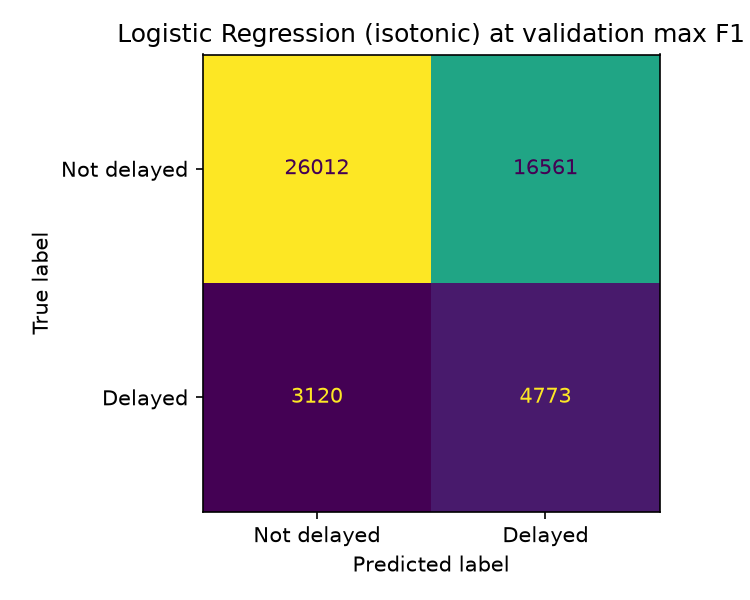
\includegraphics[width=0.49\columnwidth]{confusion-logistic}\hfill
  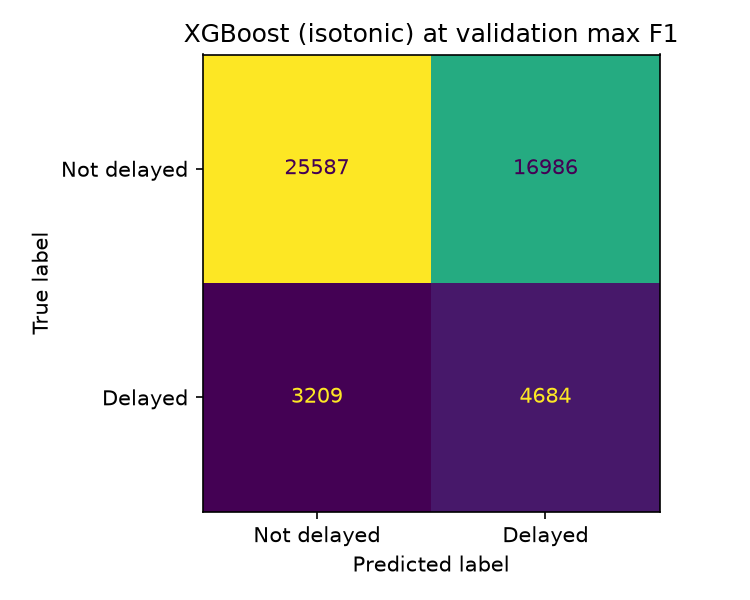
\includegraphics[width=0.49\columnwidth]{confusion-xgb}\\[2pt]
  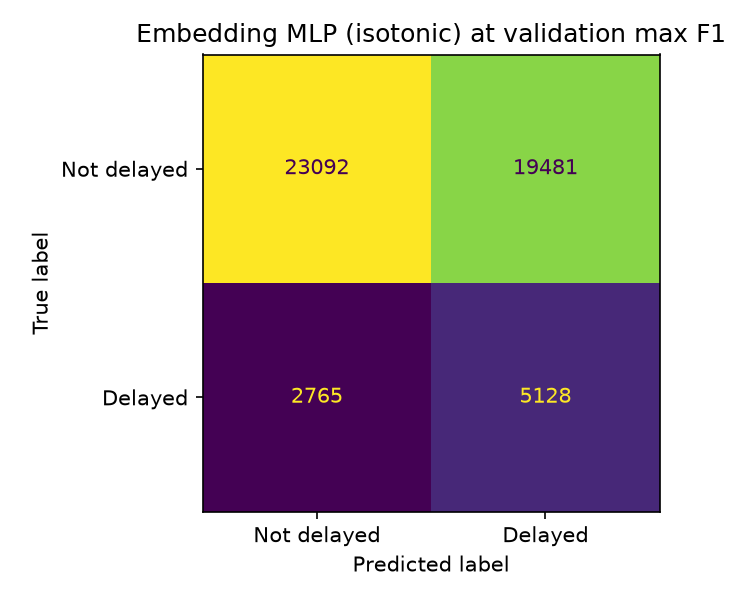
\includegraphics[width=0.49\columnwidth]{confusion-mlp}\hfill
  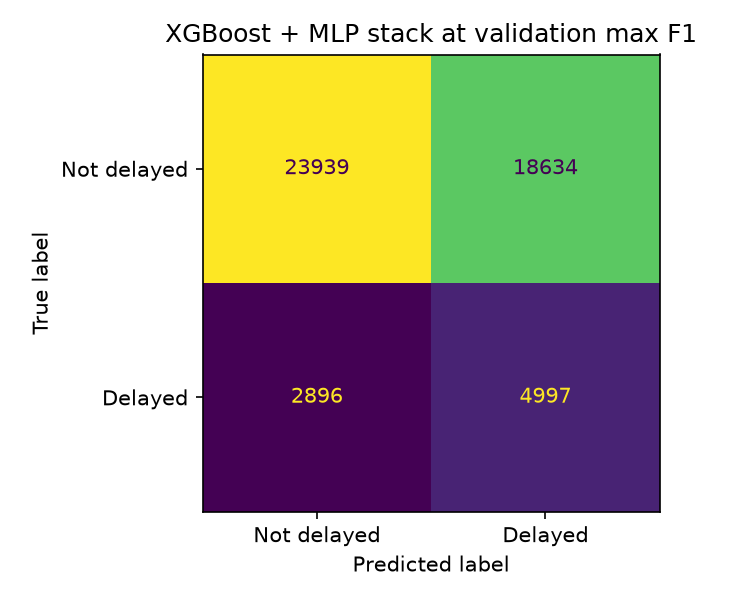
\includegraphics[width=0.49\columnwidth]{confusion-hybrid}
  \caption{Validation confusion matrices at the maximum-$F_1$ threshold for the
  calibrated Logistic Regression (top left), XGBoost (top right), embedding MLP
  (bottom left) and hybrid (bottom right). All recover most true delays at the
  cost of many false alarms (low precision).}
  \label{fig:dlconfusion}
\end{figure}

\section{Schedule-and-Route-Only Control}
\label{sec:control}
Because prior-date outcome availability at the exact decision timestamp is
unverified (Section~\ref{sec:dataset}), we refit all four candidates on only the
$23$ schedule and route predictors, dropping the eight outcome-history features,
on the same flights and windows (Table~\ref{tab:control}). Rankings are
preserved---Logistic leads, the MLP and hybrid trail slightly---and AP drops only
marginally, confirming that most of the (weak) signal is carried by schedule and
route structure that is unambiguously available pre-departure. In the same
control, an offline what-if at action-cost ratio $0.25$ and recovery $0.8$ makes
\emph{all four} policies cost more than inaction, consistent with the Phase~1
finding that model-guided rescheduling pays off only under cheap-intervention
assumptions.

\begin{table}[!t]
  \caption{Schedule-and-route-only control (23 features; isotonic).}
  \label{tab:control}
  \centering
  \begin{tabular}{lrr}
    \toprule
    Model & Validation AP & Brier \\
    \midrule
    Logistic Regression & $0.2217$ & $0.1506$ \\
    XGBoost             & $0.2116$ & $0.1370$ \\
    Embedding MLP       & $0.2075$ & $0.1386$ \\
    Hybrid (XGB$+$MLP)  & $0.2080$ & $0.1367$ \\
    \bottomrule
  \end{tabular}
\end{table}

\section{Technical Validation and Code Quality}
\label{sec:validation}
The Phase~2 work is validated rather than merely asserted.

\textbf{Unit tests and CI.}
The repository ships $28$ test files with $194$ test functions, of which $54$
(across the $6$ DL/hybrid files) cover the deep-learning path:
\code{test\_dl\_dataset}, \code{test\_dl\_encoding}, \code{test\_dl\_mlp},
\code{test\_dl\_training}, \code{test\_dl\_comparison} and \code{test\_hybrid},
with further leakage/availability checks in \code{test\_historical\_availability}
and \code{test\_frozen\_predictions}. They exercise single- and multi-flight
batches, missing and unseen IDs, gradients into each embedding table, a synthetic
carrier$\times$dense interaction the MLP must learn, outcome-perturbation leakage
checks across partition boundaries, and train-only fitting of every statistic. A
GitHub Actions workflow runs the synthetic-data tests on every push and pull
request.

\textbf{Checkpoint replay and audit.}
A verifier confirms that the committed MLP weights, preprocessing state and
dataset reproduce the saved validation probabilities within numerical tolerance
(checkpoint replay, not a full retrain). The saved hybrid outputs were
independently replayed from the reported meta-learner weights and matched all
$50{,}466$ probabilities within $1.67\times10^{-16}$ maximum absolute error. An
independent validation audit verified identical flight IDs, dates and labels
across all six committed prediction files.

\textbf{Artifact pinning.}
\code{summary.json} records the dataset SHA-256 and a per-model artifact SHA-256,
so a reviewer can confirm the reported numbers came from the committed data and
code. The evaluation writes all metrics and figures to \code{reports/dl/} and is
reproducible from the documented commands.

\section{Discussion and Limitations}
\label{sec:discussion}
Held-out discrimination is modest (test ROC-AUC $\approx 0.60$; validation
$\approx 0.62$--$0.65$). The audit did not establish a between-model difference on
the classical side or a proper-score improvement over a prevalence baseline, and
the deep models match but do not beat gradient boosting. Delay prevalence shifts
across windows (Fig.~\ref{fig:prevalence}), which limits direct comparison of AP
between partitions. The gain-importance ranking in Fig.~\ref{fig:importance}
describes the fitted XGBoost model and does not imply causation.

We disclose the following limitations: (i)~validation-only calibration and
threshold selection are not independent held-out test evidence; (ii)~the prior-day
historical protocol guarantees date ordering but not exact real-time outcome
availability; (iii)~the MLP and hybrid do not demonstrate a ranking gain over the
classical baseline on this dataset, and our negative hybrid result does not rule
out other DL architectures or representation-level fusion; (iv)~the data cover a
single year and only three New York origin airports, limiting generalisation;
(v)~the paired calendar-day bootstrap treats days as exchangeable and is
descriptive, not a serially robust confidence interval; and (vi)~no real airline
rescheduling actions or savings are verified---the offline what-if depends on
explicit, unapproved cost assumptions. None of the results supports a
production-readiness claim.

\section{Conclusion and Future Work}
\label{sec:conclusion}
We delivered a leakage-aware, calibrated and honestly evaluated classical
baseline for pre-departure flight-delay prediction---with full EDA, feature
engineering, a frozen held-out test (XGBoost the stronger candidate at test AP
$0.337$), feature importance, and an offline cost-sensitive rescheduling
analysis---and then built and rigorously evaluated a deep learning extension
measured against it: an entity-embedding MLP and a stacked XGBoost$+$MLP hybrid,
scored on the same $50{,}466$ validation flights under identical leakage
controls. The MLP produces valid, well-behaved and (after isotonic calibration)
competitively calibrated probabilities, but it does not out-rank gradient
boosting, and the hybrid adds no ranking value because the two models' residuals
are $0.968$-correlated and the meta-learner collapses onto XGBoost. Every number
is explained by a cause we can point to---a weak pre-departure signal (hence
modest ROC-AUC, best epoch~1, and unattainable high-precision operating points), a
prevalence shift (hence residual over-prediction), and redundant base learners
(hence the null hybrid). This is the behaviour the tabular-deep-learning
literature predicts, and we present it as a reproducible, well-instrumented
negative/ablation contribution. The natural next steps are the larger BTS on-time
dataset for a sterner generalisation test, and representation-level ML$+$DL
fusion, which the measured error diversity suggests will yield only limited gains
on this problem.

\section*{Reproducibility}
Continuous integration tests the classical and CPU PyTorch paths. The frozen
evaluation records dataset and artifact SHA-256 hashes and dependency versions.
The Phase~2 checkpoint verifier reproduced all $50{,}466$ validation
probabilities exactly. The repository includes prediction CSVs, matched-seed
runs, the presentation, and a demonstration guide.

\section*{Team Contributions}
Lakshya integrated the dataset adapter and audited historical availability.
Ankit Raj Singh implemented categorical encoding and the embedding tables.
Samiksha Jangid implemented the embedding MLP and its architecture tests.
Rashmi Anand implemented training, tuning and checkpoint export.
Shubhaang Kataruka implemented the AML--DL comparison, the hybrid stack and the
checkpoint audit.

\section*{Acknowledgment}
This Phase~2 work builds directly on the Phase~1 machine-learning pipeline and on
the course's deep-learning lecture and lab materials~\cite{dl-notes,dl-lab}, with
the advanced-machine-learning lecture and lab notes~\cite{aml-notes,aml-lab}
underpinning the classical baseline. We additionally used the AI assistants
ChatGPT~\cite{chatgpt} and Claude~\cite{claude} for drafting and debugging
support; all modelling decisions, code, experiments and results were authored and
verified by the team.

\begin{thebibliography}{00}
\bibitem{dl-notes} Deep Learning lecture notes (course material).
\bibitem{dl-lab} Deep Learning lab notes (course material).
\bibitem{aml-notes} Advanced Machine Learning lecture notes (course material).
\bibitem{aml-lab} Advanced Machine Learning lab notes (course material).
\bibitem{kaggle} M. Sajadi, ``Flights,'' Kaggle. [Online]. Available: \url{https://www.kaggle.com/datasets/matinsajadi/flights}.
\bibitem{chatgpt} OpenAI, ChatGPT. [Online]. Available: \url{https://chatgpt.com/}.
\bibitem{claude} Anthropic, Claude. [Online]. Available: \url{https://claude.ai/}.
\bibitem{entityembed} C. Guo and F. Berkhahn, ``Entity Embeddings of Categorical Variables,'' \emph{arXiv:1604.06737}, 2016.
\bibitem{guo} C. Guo, G. Pleiss, Y. Sun, and K. Q. Weinberger, ``On Calibration of Modern Neural Networks,'' in \emph{Proc.\ ICML}, 2017, pp.\ 1321--1330.
\bibitem{grinsztajn} L. Grinsztajn, E. Oyallon, and G. Varoquaux, ``Why do tree-based models still outperform deep learning on tabular data?,'' \emph{arXiv:2207.08815}, 2022.
\bibitem{shwartzziv} R. Shwartz-Ziv and A. Armon, ``Tabular Data: Deep Learning is Not All You Need,'' \emph{arXiv:2106.03253}, 2021.
\bibitem{fbgbdt} X. He \emph{et al.}, ``Practical Lessons from Predicting Clicks on Ads at Facebook,'' in \emph{Proc.\ ADKDD}, 2014, pp.\ 1--9.
\bibitem{bts} U.S. Bureau of Transportation Statistics, ``Airline On-Time Performance Data,'' TranStats database. [Online]. Available: \url{https://www.transtats.bts.gov/}.
\end{thebibliography}

\end{document}
